\chapter{IOZone benchmarking data}
\label{app:bench_data}

This appendix contains tables of the IOZone benchmarking outputs produced. Each section contains the raw table output for the benchmarking results of the specific filesystem. Each table represents one IOZone test for a filesystem. Each table presents the throughput in kilobytes per second for a test, for the different file sizes and buffer sizes, both presented in kB.

\section{FFS}

\begin{table}[!ht]
	\begin{center}
		\caption{IOZone result for the Read test on FFS in kilobytes per second}
		\resizebox{\textwidth}{!}{\begin{tabular}{| r | r | r | r | r | r | r | r | r | r | r | r | r | r | }
			
			\hline
			{} & \multicolumn{13}{c |}{Buffer size (kB)} \\
			\textbf{File size (kB)}   & \multicolumn{1}{c |}{4} & \multicolumn{1}{c |}{8} & \multicolumn{1}{c |}{16} & \multicolumn{1}{c |}{32} & \multicolumn{1}{c |}{64} & \multicolumn{1}{c |}{128} & \multicolumn{1}{c |}{256} & \multicolumn{1}{c |}{512} & \multicolumn{1}{c |}{1024} & \multicolumn{1}{c |}{2048} & \multicolumn{1}{c |}{4096} & \multicolumn{1}{c |}{8192} & \multicolumn{1}{c |}{16384}\\
			\hline
			\hline
			\textbf{1024}  & 1124099 & 1875690 & 2072054 & 2606476 & 2386350 & 2844715 & 2604895 & 2173780 & 3210456 & {} & {} & {} & {}\\
			\textbf{2048}  & 1378181 & 567636 & 2033695 & 2972495 & 3154809 & 3121562 & 3690142 & 2301200 & 3519302 & 2235910 & {} & {} & {}\\
			\textbf{4096}  & 1614527 & 2298370 & 2955012 & 4027344 & 4628439 & 3942321 & 4511750 & 4007615 & 4329816 & 4095510 & 3953206 & {} & {}\\
			\textbf{8192}  & 2021184 & 2978787 & 3852936 & 5329730 & 3541581 & 3591558 & 4638941 & 6390362 & 3444652 & 5919188 & 4003788 & 5095007 & {}\\
			\textbf{16384}  & 60625 & 2246482 & 63191 & 4702688 & 61471 & 6206148 & 2936754 & 6362439 & 69217 & 5168507 & 2375140 & 117941 & 4462939\\
			\textbf{32768}  & 55818 & 52177 & 4466247 & 5033507 & 60178 & 54036 & 35729 & 54242 & 5819047 & 53512 & 5501562 & 64800 & 86733\\
			\textbf{65536}  & 124344 & 50556 & 54524 & 52190 & 4810367 & 67341 & 53582 & 50273 & 52437 & 4826246 & 56654 & 56309 & 4882655\\
			\textbf{131072}  & 2973359 & 4220618 & 68079 & 70359 & 69429 & 7874149 & 60407 & 70434 & 7260 & 81991 & 62072 & 6522596 & 79478\\
			\textbf{262144}  & 68103 & 70685 & 68449 & 69849 & 99154 & 70227 & 68031 & 71294 & 68417 & 59723 & 7519272 & 6089594 & 161814\\


			\hline

		\end{tabular}}
		\label{tbl:data_ffs_read}
	\end{center}
\end{table}
	
\begin{table}[!ht]
	\begin{center}
		\caption{IOZone result for the Write test on FFS in kilobytes per second}
		\resizebox{\textwidth}{!}{\begin{tabular}{| r | r | r | r | r | r | r | r | r | r | r | r | r | r | }
			
			\hline
			{} & \multicolumn{13}{c |}{Buffer size (kB)} \\
			\textbf{File size (kB)}   & \multicolumn{1}{c |}{4} & \multicolumn{1}{c |}{8} & \multicolumn{1}{c |}{16} & \multicolumn{1}{c |}{32} & \multicolumn{1}{c |}{64} & \multicolumn{1}{c |}{128} & \multicolumn{1}{c |}{256} & \multicolumn{1}{c |}{512} & \multicolumn{1}{c |}{1024} & \multicolumn{1}{c |}{2048} & \multicolumn{1}{c |}{4096} & \multicolumn{1}{c |}{8192} & \multicolumn{1}{c |}{16384}\\
			\hline
			\hline
			\textbf{1024}  & 206 & 270 & 312 & 271 & 262 & 319 & 248 & 310 & 325 & {} & {} & {} & {}\\
			\textbf{2048}  & 492 & 447 & 486 & 441 & 532 & 458 & 496 & 506 & 536 & 504 & {} & {} & {}\\
			\textbf{4096}  & 774 & 803 & 686 & 853 & 816 & 846 & 829 & 746 & 738 & 816 & 839 & {} & {}\\
			\textbf{8192}  & 1099 & 640 & 1236 & 1056 & 1054 & 1095 & 1078 & 975 & 1177 & 1068 & 1029 & 1077 & {}\\
			\textbf{16384}  & 1320 & 1240 & 1369 & 1344 & 1413 & 1363 & 1339 & 1278 & 1349 & 1427 & 1341 & 1344 & 1187\\
			\textbf{32768}  & 1573 & 1749 & 1685 & 1625 & 1610 & 1647 & 1639 & 1750 & 1745 & 1734 & 1636 & 1650 & 1727\\
			\textbf{65536}  & 1875 & 1995 & 2062 & 1724 & 2029 & 1995 & 1783 & 2007 & 2008 & 2052 & 2109 & 1955 & 2068\\
			\textbf{131072}  & 2059 & 2297 & 2472 & 2154 & 2176 & 2362 & 2236 & 2465 & 2433 & 2393 & 2644 & 2474 & 2384\\
			\textbf{262144}  & 2339 & 2139 & 2597 & 2157 & 2529 & 2421 & 548 & 894 & 2623 & 2612 & 2676 & 2637 & 2646\\


			\hline

		\end{tabular}}
		\label{tbl:data_ffs_write}
	\end{center}
\end{table}
	
\begin{table}[!ht]
	\begin{center}
		\caption{IOZone result for the Re-Read test on FFS in kilobytes per second}
		\resizebox{\textwidth}{!}{\begin{tabular}{| r | r | r | r | r | r | r | r | r | r | r | r | r | r | }
			
			\hline
			{} & \multicolumn{13}{c |}{Buffer size (kB)} \\
			\textbf{File size (kB)}   & \multicolumn{1}{c |}{4} & \multicolumn{1}{c |}{8} & \multicolumn{1}{c |}{16} & \multicolumn{1}{c |}{32} & \multicolumn{1}{c |}{64} & \multicolumn{1}{c |}{128} & \multicolumn{1}{c |}{256} & \multicolumn{1}{c |}{512} & \multicolumn{1}{c |}{1024} & \multicolumn{1}{c |}{2048} & \multicolumn{1}{c |}{4096} & \multicolumn{1}{c |}{8192} & \multicolumn{1}{c |}{16384}\\
			\hline
			\hline
			\textbf{1024}  & 1025833 & 2056183 & 1600327 & 2789291 & 2966535 & 2625597 & 3020783 & 2976816 & 4178773 & {} & {} & {} & {}\\
			\textbf{2048}  & 2183619 & 1430271 & 2595298 & 2418469 & 3675930 & 2748949 & 4762117 & 3272598 & 3555722 & 3117032 & {} & {} & {}\\
			\textbf{4096}  & 2326065 & 2740095 & 3093350 & 4218190 & 4298399 & 4735608 & 5618365 & 5483860 & 5704175 & 3419011 & 4321103 & {} & {}\\
			\textbf{8192}  & 2185761 & 3618412 & 4754484 & 5197511 & 4250966 & 6248582 & 6725591 & 6522590 & 4385525 & 6765318 & 4771651 & 4445097 & {}\\
			\textbf{16384}  & 1841910 & 2301789 & 4900900 & 5791387 & 6534875 & 6582447 & 6852209 & 6427904 & 7599353 & 3720236 & 5858035 & 4687931 & 4717539\\
			\textbf{32768}  & 2375173 & 3448145 & 4222679 & 5487065 & 6201613 & 6714556 & 5137750 & 6366213 & 6636098 & 6273801 & 5597460 & 5099433 & 5232021\\
			\textbf{65536}  & 1777628 & 3099807 & 3788868 & 5457737 & 4664497 & 5469466 & 7114221 & 6547080 & 6423160 & 5395284 & 5009273 & 4816014 & 4676161\\
			\textbf{131072}  & 2666778 & 3783414 & 5009036 & 6003942 & 6385321 & 8230640 & 6553543 & 7089250 & 6747555 & 6880134 & 5982251 & 6600438 & 6078894\\
			\textbf{262144}  & 2583743 & 4449684 & 5590363 & 6013557 & 6771275 & 6868693 & 7097066 & 7641769 & 7053902 & 7329012 & 4997807 & 4674122 & 5487959\\


			\hline

		\end{tabular}}
		\label{tbl:data_ffs_re-read}
	\end{center}
\end{table}
	
\begin{table}[!ht]
	\begin{center}
		\caption{IOZone result for the Re-Write test on FFS in kilobytes per second}
		\resizebox{\textwidth}{!}{\begin{tabular}{| r | r | r | r | r | r | r | r | r | r | r | r | r | r | }
			
			\hline
			{} & \multicolumn{13}{c |}{Buffer size (kB)} \\
			\textbf{File size (kB)}   & \multicolumn{1}{c |}{4} & \multicolumn{1}{c |}{8} & \multicolumn{1}{c |}{16} & \multicolumn{1}{c |}{32} & \multicolumn{1}{c |}{64} & \multicolumn{1}{c |}{128} & \multicolumn{1}{c |}{256} & \multicolumn{1}{c |}{512} & \multicolumn{1}{c |}{1024} & \multicolumn{1}{c |}{2048} & \multicolumn{1}{c |}{4096} & \multicolumn{1}{c |}{8192} & \multicolumn{1}{c |}{16384}\\
			\hline
			\hline
			\textbf{1024}  & 256 & 246 & 200 & 264 & 308 & 269 & 250 & 293 & 324 & {} & {} & {} & {}\\
			\textbf{2048}  & 532 & 511 & 404 & 547 & 505 & 533 & 564 & 489 & 434 & 457 & {} & {} & {}\\
			\textbf{4096}  & 864 & 768 & 775 & 826 & 762 & 793 & 880 & 767 & 787 & 835 & 721 & {} & {}\\
			\textbf{8192}  & 942 & 930 & 958 & 935 & 896 & 1006 & 895 & 863 & 942 & 862 & 959 & 943 & {}\\
			\textbf{16384}  & 1155 & 1100 & 1113 & 1147 & 1141 & 1130 & 1106 & 1160 & 1048 & 1160 & 1137 & 1089 & 1111\\
			\textbf{32768}  & 1327 & 1357 & 1335 & 1423 & 1350 & 1387 & 1363 & 1351 & 1296 & 1411 & 1245 & 1390 & 1282\\
			\textbf{65536}  & 1447 & 1542 & 1534 & 1474 & 1420 & 1632 & 1412 & 1661 & 1579 & 1585 & 1599 & 1679 & 1637\\
			\textbf{131072}  & 1729 & 1813 & 1637 & 1641 & 1567 & 1748 & 1716 & 1963 & 1945 & 1936 & 1902 & 1954 & 1885\\
			\textbf{262144}  & 1822 & 1823 & 1944 & 1949 & 1939 & 1995 & 1940 & 1983 & 2009 & 1967 & 1987 & 2000 & 1992\\


			\hline

		\end{tabular}}
		\label{tbl:data_ffs_re-write}
	\end{center}
\end{table}
	
\begin{table}[!ht]
	\begin{center}
		\caption{IOZone result for the Random read test on FFS in kilobytes per second}
		\resizebox{\textwidth}{!}{\begin{tabular}{| r | r | r | r | r | r | r | r | r | r | r | r | r | r | }
			
			\hline
			{} & \multicolumn{13}{c |}{Buffer size (kB)} \\
			\textbf{File size (kB)}   & \multicolumn{1}{c |}{4} & \multicolumn{1}{c |}{8} & \multicolumn{1}{c |}{16} & \multicolumn{1}{c |}{32} & \multicolumn{1}{c |}{64} & \multicolumn{1}{c |}{128} & \multicolumn{1}{c |}{256} & \multicolumn{1}{c |}{512} & \multicolumn{1}{c |}{1024} & \multicolumn{1}{c |}{2048} & \multicolumn{1}{c |}{4096} & \multicolumn{1}{c |}{8192} & \multicolumn{1}{c |}{16384}\\
			\hline
			\hline
			\textbf{1024}  & 157493 & 2216407 & 1627617 & 1741810 & 2852271 & 2926114 & 3722435 & 2275110 & 4146499 & {} & {} & {} & {}\\
			\textbf{2048}  & 1782585 & 416667 & 2916978 & 2752473 & 3379461 & 4031308 & 2763987 & 3624742 & 4265523 & 3894239 & {} & {} & {}\\
			\textbf{4096}  & 1536962 & 2719708 & 2965725 & 4270618 & 3497668 & 5411313 & 3918939 & 5360658 & 4409837 & 4302706 & 4707064 & {} & {}\\
			\textbf{8192}  & 1719637 & 2589902 & 4021596 & 4670469 & 4928384 & 6420214 & 6703285 & 6996761 & 4528880 & 5978928 & 4879393 & 4551075 & {}\\
			\textbf{16384}  & 1790371 & 1826537 & 4196659 & 4780882 & 4288854 & 5544663 & 6963302 & 6863844 & 7133159 & 4528524 & 4973975 & 4546200 & 4920199\\
			\textbf{32768}  & 1652689 & 2699602 & 3615596 & 5126252 & 5529450 & 5983722 & 5242798 & 6766123 & 5356822 & 5140824 & 5706695 & 5170803 & 2796839\\
			\textbf{65536}  & 1361645 & 2149636 & 3197042 & 4471609 & 4626031 & 5484198 & 6721584 & 6197810 & 6846648 & 3663045 & 4794509 & 5149377 & 4639069\\
			\textbf{131072}  & 1971894 & 3118619 & 3812353 & 5415790 & 6283727 & 7615527 & 5731410 & 7322871 & 6164024 & 6919971 & 5118969 & 4799231 & 5960782\\
			\textbf{262144}  & 1813113 & 3068092 & 3975558 & 4985728 & 6536121 & 6311675 & 6655244 & 7390988 & 7063782 & 7242548 & 6004755 & 5722694 & 5567942\\


			\hline

		\end{tabular}}
		\label{tbl:data_ffs_random_read}
	\end{center}
\end{table}
	
\begin{table}[!ht]
	\begin{center}
		\caption{IOZone result for the Random write test on FFS in kilobytes per second}
		\resizebox{\textwidth}{!}{\begin{tabular}{| r | r | r | r | r | r | r | r | r | r | r | r | r | r | }
			
			\hline
			{} & \multicolumn{13}{c |}{Buffer size (kB)} \\
			\textbf{File size (kB)}   & \multicolumn{1}{c |}{4} & \multicolumn{1}{c |}{8} & \multicolumn{1}{c |}{16} & \multicolumn{1}{c |}{32} & \multicolumn{1}{c |}{64} & \multicolumn{1}{c |}{128} & \multicolumn{1}{c |}{256} & \multicolumn{1}{c |}{512} & \multicolumn{1}{c |}{1024} & \multicolumn{1}{c |}{2048} & \multicolumn{1}{c |}{4096} & \multicolumn{1}{c |}{8192} & \multicolumn{1}{c |}{16384}\\
			\hline
			\hline
			\textbf{1024}  & 230 & 255 & 264 & 338 & 287 & 304 & 184 & 317 & 289 & {} & {} & {} & {}\\
			\textbf{2048}  & 524 & 431 & 462 & 512 & 468 & 513 & 570 & 492 & 446 & 558 & {} & {} & {}\\
			\textbf{4096}  & 822 & 857 & 787 & 688 & 811 & 799 & 791 & 815 & 793 & 766 & 828 & {} & {}\\
			\textbf{8192}  & 907 & 917 & 861 & 865 & 993 & 977 & 747 & 904 & 913 & 918 & 929 & 972 & {}\\
			\textbf{16384}  & 1021 & 1013 & 1197 & 1126 & 1170 & 1127 & 1163 & 1031 & 1119 & 1138 & 1036 & 1180 & 1057\\
			\textbf{32768}  & 1297 & 1268 & 1299 & 1405 & 1314 & 1310 & 1238 & 1210 & 1326 & 1297 & 1298 & 1334 & 1322\\
			\textbf{65536}  & 1375 & 1384 & 1634 & 1522 & 1591 & 1587 & 1671 & 1606 & 1608 & 1634 & 1597 & 1624 & 1627\\
			\textbf{131072}  & 1605 & 1784 & 1797 & 1715 & 1595 & 1631 & 1960 & 1910 & 1842 & 2001 & 1922 & 1935 & 1929\\
			\textbf{262144}  & 1793 & 1945 & 1870 & 1987 & 2005 & 1962 & 1952 & 1999 & 1782 & 1988 & 2019 & 2014 & 2034\\


			\hline

		\end{tabular}}
		\label{tbl:data_ffs_random_write}
	\end{center}
\end{table}
	

\FloatBarrier

% \begin{figure}[!htb]
% 	\label{fig:app_bench_ffs_read}
% 	\begin{center}
% 		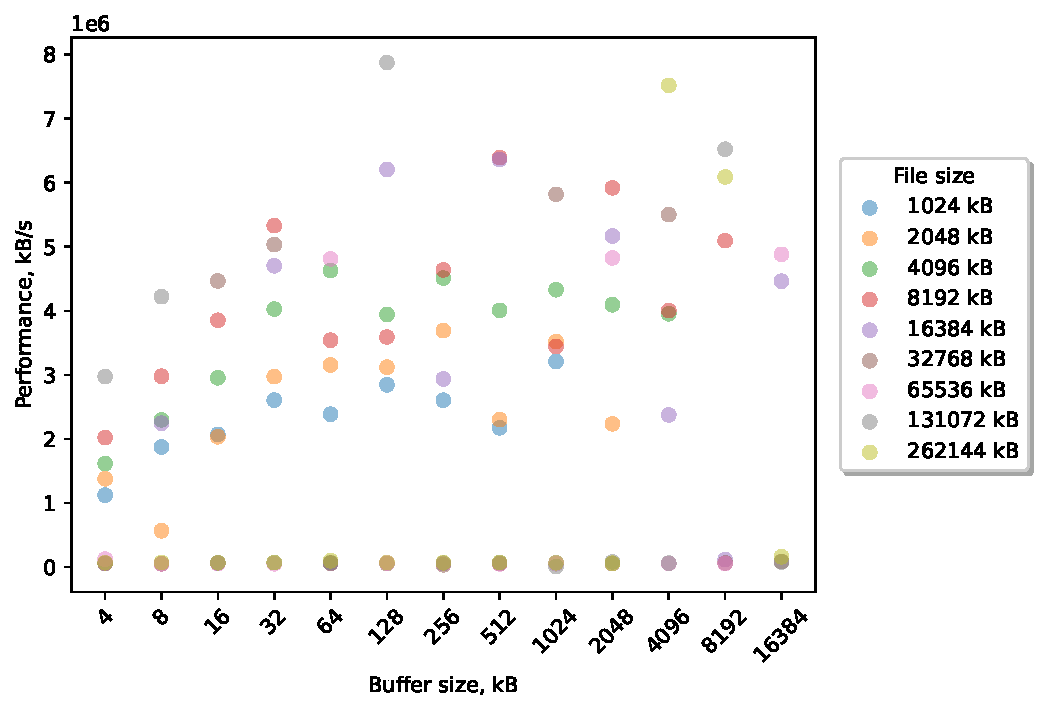
\includegraphics[width=1.0\textwidth]{figures.nosync/benchmarking/old/ffs/Read.pdf}
% 	\end{center}
% 	\caption{IOZone output for FFS Forward Read}
% \end{figure}

% \begin{figure}[!htb]
% 	\label{fig:app_bench_ffs_write}
% 	\begin{center}
% 		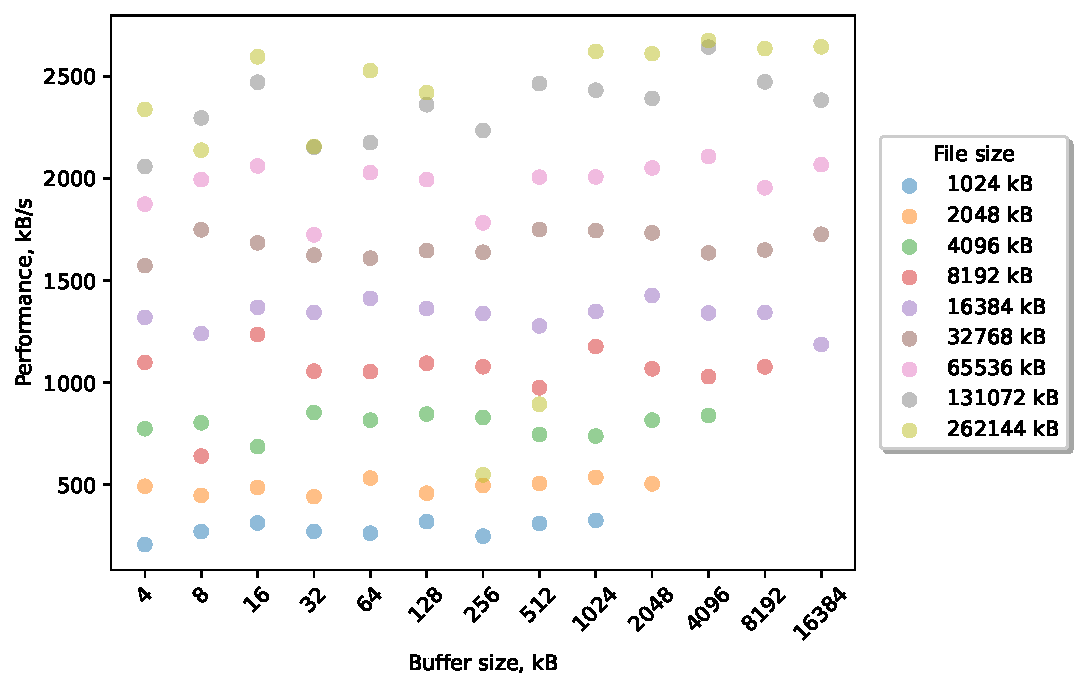
\includegraphics[width=1.0\textwidth]{figures.nosync/benchmarking/old/ffs/Write.pdf}
% 	\end{center}
% 	\caption{IOZone output for FFS Forward Write}
% \end{figure}

% \begin{figure}[!htb]
% 	\label{fig:app_bench_ffs_re_read}
% 	\begin{center}
% 		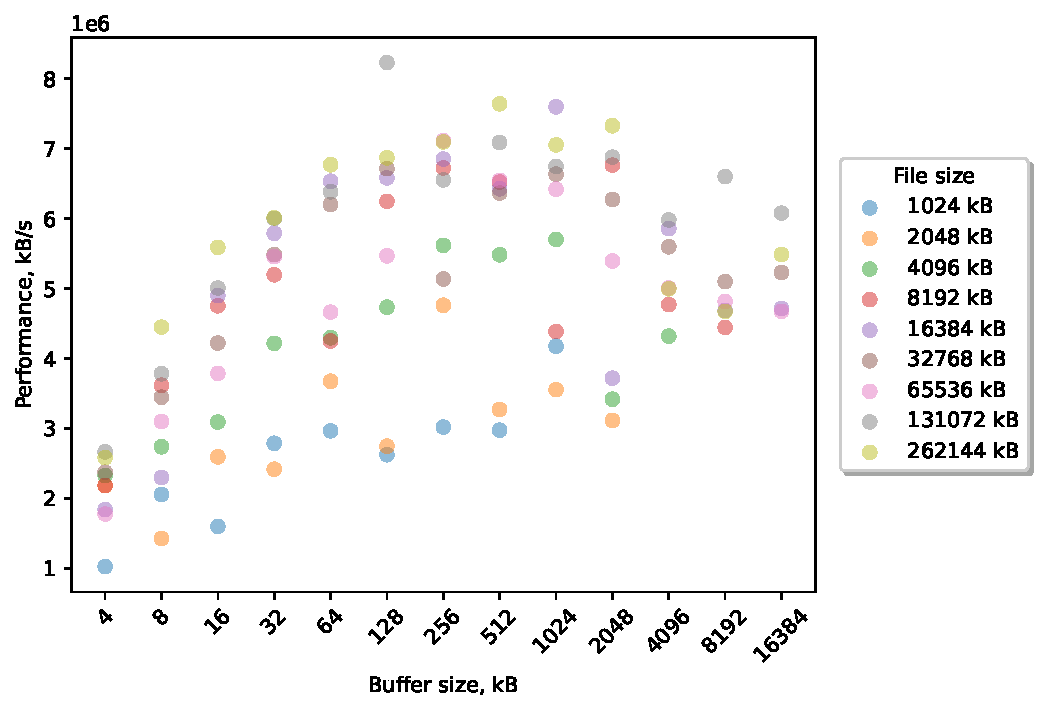
\includegraphics[width=1.0\textwidth]{figures.nosync/benchmarking/old/ffs/Re-Read.pdf}
% 	\end{center}
% 	\caption{IOZone output for FFS \mbox{Re-Read}}
% \end{figure}

% \begin{figure}[!htb]
% 	\label{fig:app_bench_ffs_re_write}
% 	\begin{center}
% 		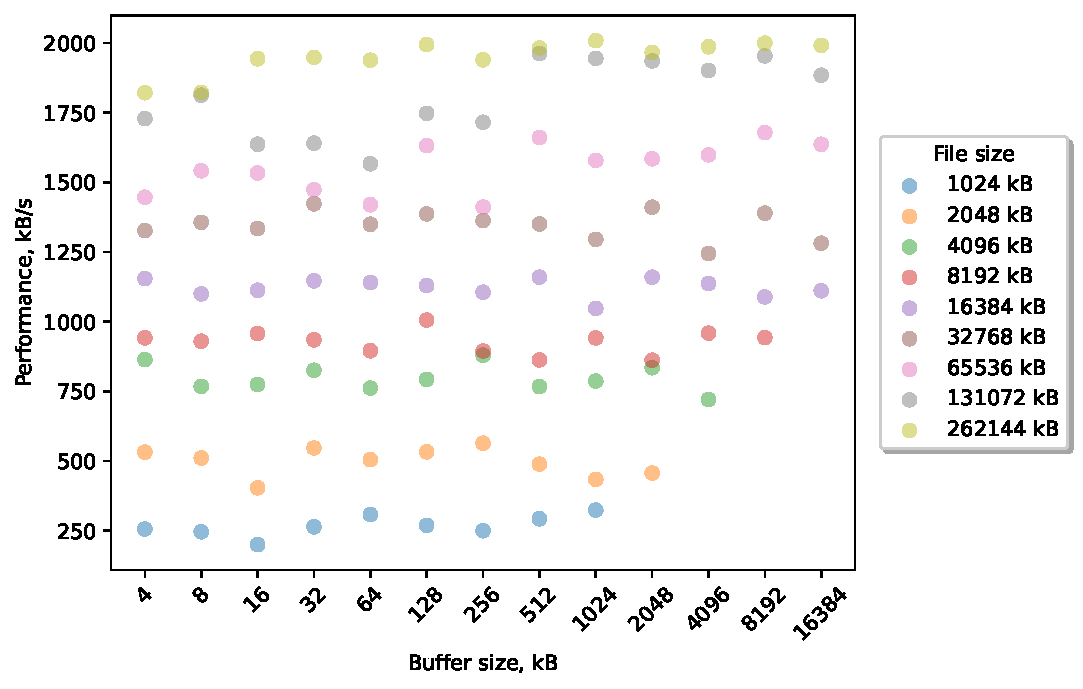
\includegraphics[width=1.0\textwidth]{figures.nosync/benchmarking/old/ffs/Re-Write.pdf}
% 	\end{center}
% 	\caption{IOZone output for FFS \mbox{Re-Write}}
% \end{figure}

% \begin{figure}[!htb]
% 	\label{fig:app_bench_ffs_rnd_read}
% 	\begin{center}
% 		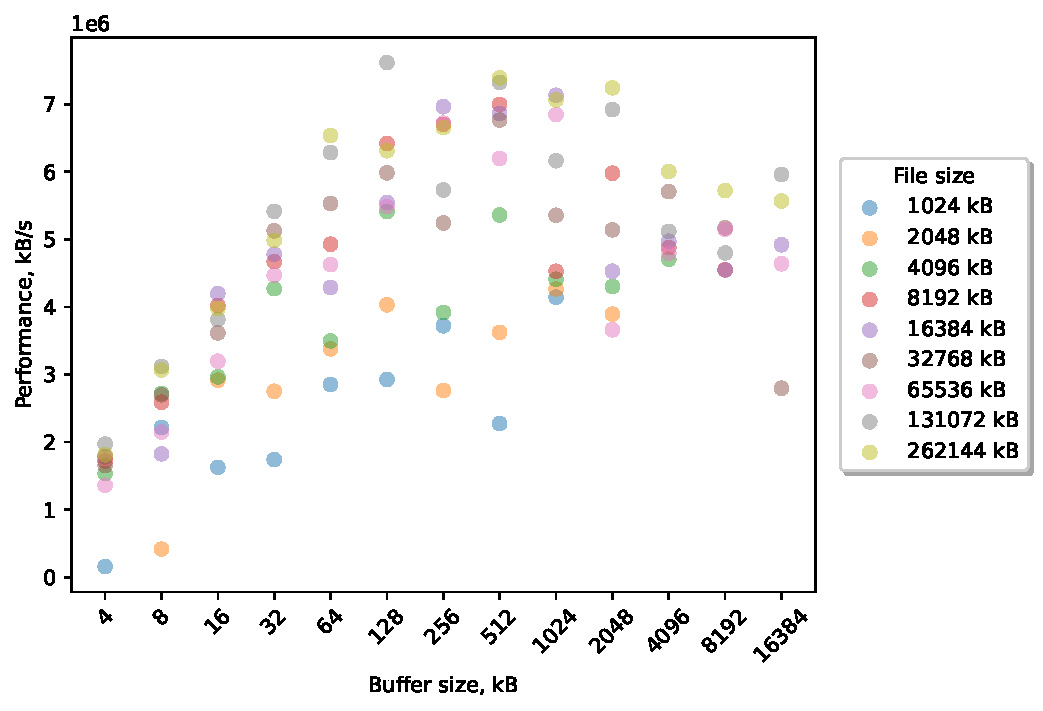
\includegraphics[width=1.0\textwidth]{figures.nosync/benchmarking/old/ffs/Random read.pdf}
% 	\end{center}
% 	\caption{IOZone output for FFS Random read}
% \end{figure}

% \begin{figure}[!htb]
% 	\label{fig:app_bench_ffs_rnd_write}
% 	\begin{center}
% 		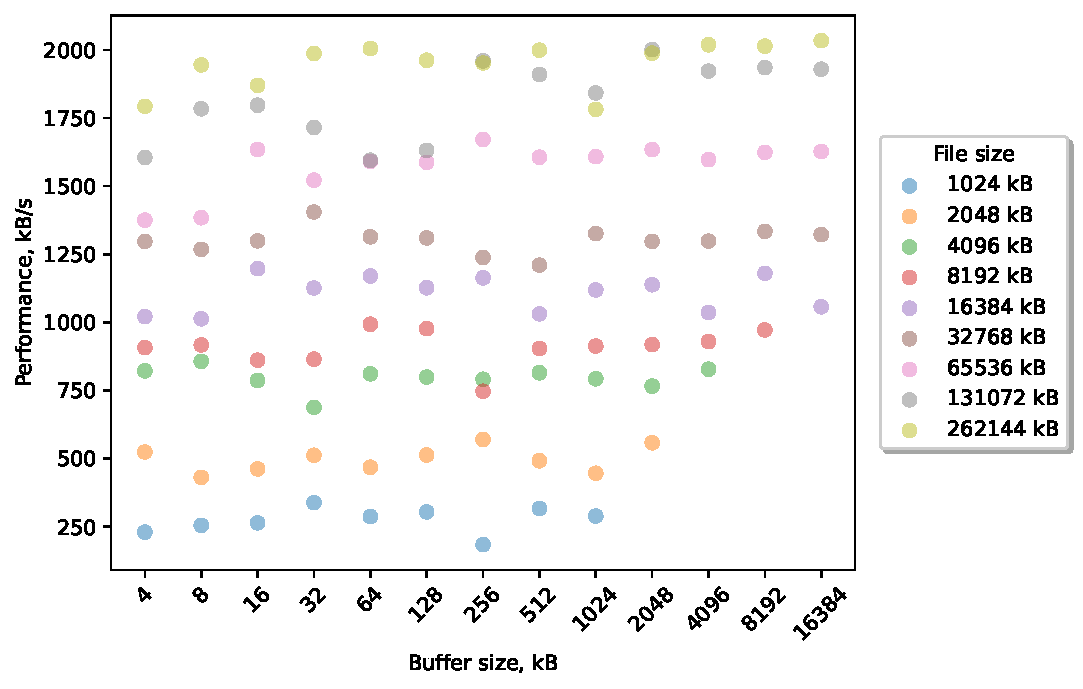
\includegraphics[width=1.0\textwidth]{figures.nosync/benchmarking/old/ffs/Random write.pdf}
% 	\end{center}
% 	\caption{IOZone output for FFS Random write}
% \end{figure}

\newpage

\section{GCSF}

\begin{table}[!ht]
	\begin{center}
		\caption{IOZone result for the Read test on GCSF in kilobytes per second}
		\resizebox{\textwidth}{!}{\begin{tabular}{| r | r | r | r | r | r | r | r | r | r | r | r | r | r | }
			
			\hline
			{} & \multicolumn{13}{c |}{Buffer size (kB)} \\
			\textbf{File size (kB)}   & \multicolumn{1}{c |}{4} & \multicolumn{1}{c |}{8} & \multicolumn{1}{c |}{16} & \multicolumn{1}{c |}{32} & \multicolumn{1}{c |}{64} & \multicolumn{1}{c |}{128} & \multicolumn{1}{c |}{256} & \multicolumn{1}{c |}{512} & \multicolumn{1}{c |}{1024} & \multicolumn{1}{c |}{2048} & \multicolumn{1}{c |}{4096} & \multicolumn{1}{c |}{8192} & \multicolumn{1}{c |}{16384}\\
			\hline
			\hline
			\textbf{1024}  & 1790460 & 2035716 & 2753527 & 3411938 & 3003881 & 3401130 & 3722435 & 4162573 & 4493556 & {} & {} & {} & {}\\
			\textbf{2048}  & 945007 & 2308622 & 3297725 & 4170264 & 3698085 & 2467800 & 3506373 & 4611288 & 5416763 & 4376355 & {} & {} & {}\\
			\textbf{4096}  & 1858527 & 2813233 & 1017897 & 4969868 & 4399673 & 4941279 & 4591331 & 5657217 & 5625724 & 5019235 & 3327622 & {} & {}\\
			\textbf{8192}  & 651866 & 480214 & 4126896 & 4664763 & 903994 & 5357988 & 3195123 & 5288712 & 6804170 & 1412655 & 4833405 & 5085204 & {}\\
			\textbf{16384}  & 409261 & 3463891 & 4768276 & 518677 & 5797739 & 6450228 & 6077171 & 6143453 & 6930296 & 6316241 & 5948808 & 837411 & 5326345\\
			\textbf{32768}  & 289995 & 2604351 & 514007 & 5222875 & 351689 & 380969 & 225834 & 428160 & 377558 & 3011251 & 422812 & 601160 & 710955\\
			\textbf{65536}  & 420968 & 390311 & 374191 & 590919 & 6243421 & 863782 & 388813 & 506734 & 463735 & 478777 & 456922 & 429282 & 624033\\
			\textbf{131072}  & 443068 & 462364 & 407350 & 496836 & 444001 & 471616 & 424145 & 518826 & 505112 & 559713 & 375452 & 526586 & 515828\\


			\hline

		\end{tabular}}
		\label{tbl:data_gcsf_read}
	\end{center}
\end{table}
	
\begin{table}[!ht]
	\begin{center}
		\caption{IOZone result for the Write test on GCSF in kilobytes per second}
		\resizebox{\textwidth}{!}{\begin{tabular}{| r | r | r | r | r | r | r | r | r | r | r | r | r | r | }
			
			\hline
			{} & \multicolumn{13}{c |}{Buffer size (kB)} \\
			\textbf{File size (kB)}   & \multicolumn{1}{c |}{4} & \multicolumn{1}{c |}{8} & \multicolumn{1}{c |}{16} & \multicolumn{1}{c |}{32} & \multicolumn{1}{c |}{64} & \multicolumn{1}{c |}{128} & \multicolumn{1}{c |}{256} & \multicolumn{1}{c |}{512} & \multicolumn{1}{c |}{1024} & \multicolumn{1}{c |}{2048} & \multicolumn{1}{c |}{4096} & \multicolumn{1}{c |}{8192} & \multicolumn{1}{c |}{16384}\\
			\hline
			\hline
			\textbf{1024}  & 489 & 517 & 445 & 461 & 399 & 496 & 509 & 448 & 529 & {} & {} & {} & {}\\
			\textbf{2048}  & 937 & 966 & 854 & 944 & 1072 & 966 & 944 & 954 & 868 & 969 & {} & {} & {}\\
			\textbf{4096}  & 1609 & 1614 & 1749 & 1607 & 1213 & 1787 & 1802 & 1519 & 1748 & 1551 & 1784 & {} & {}\\
			\textbf{8192}  & 3047 & 2233 & 2746 & 3115 & 2666 & 2636 & 3000 & 2974 & 3165 & 2716 & 3138 & 3122 & {}\\
			\textbf{16384}  & 4372 & 4180 & 4437 & 4690 & 4798 & 4642 & 4429 & 4781 & 4705 & 4670 & 4621 & 4875 & 4607\\
			\textbf{32768}  & 5377 & 6125 & 6471 & 6402 & 6343 & 6463 & 6435 & 6289 & 5865 & 6052 & 6317 & 6291 & 6018\\
			\textbf{65536}  & 6763 & 7448 & 7298 & 7825 & 6561 & 7061 & 7818 & 6959 & 7491 & 7706 & 5985 & 7343 & 6851\\
			\textbf{131072}  & 7276 & 7789 & 8553 & 8609 & 8243 & 8596 & 8168 & 8530 & 8596 & 8433 & 8029 & 8280 & 7959\\


			\hline

		\end{tabular}}
		\label{tbl:data_gcsf_write}
	\end{center}
\end{table}
	
\begin{table}[!ht]
	\begin{center}
		\caption{IOZone result for the Re-Read test on GCSF in kilobytes per second}
		\resizebox{\textwidth}{!}{\begin{tabular}{| r | r | r | r | r | r | r | r | r | r | r | r | r | r | }
			
			\hline
			{} & \multicolumn{13}{c |}{Buffer size (kB)} \\
			\textbf{File size (kB)}   & \multicolumn{1}{c |}{4} & \multicolumn{1}{c |}{8} & \multicolumn{1}{c |}{16} & \multicolumn{1}{c |}{32} & \multicolumn{1}{c |}{64} & \multicolumn{1}{c |}{128} & \multicolumn{1}{c |}{256} & \multicolumn{1}{c |}{512} & \multicolumn{1}{c |}{1024} & \multicolumn{1}{c |}{2048} & \multicolumn{1}{c |}{4096} & \multicolumn{1}{c |}{8192} & \multicolumn{1}{c |}{16384}\\
			\hline
			\hline
			\textbf{1024}  & 2632033 & 2187063 & 3200886 & 4304412 & 3348104 & 3778101 & 3281592 & 5048117 & 4083422 & {} & {} & {} & {}\\
			\textbf{2048}  & 2311728 & 3261415 & 4623699 & 4643695 & 4079167 & 4349761 & 6149699 & 6058611 & 7213548 & 5032754 & {} & {} & {}\\
			\textbf{4096}  & 2356697 & 2579635 & 4329816 & 5424983 & 5347310 & 6309619 & 4371684 & 6585338 & 6894546 & 6370451 & 5165626 & {} & {}\\
			\textbf{8192}  & 1891555 & 3974610 & 4017834 & 4884942 & 6112956 & 6262248 & 5158495 & 5116249 & 7087688 & 6720329 & 5270864 & 5038228 & {}\\
			\textbf{16384}  & 2228199 & 3960364 & 5075741 & 6187150 & 6473317 & 6838571 & 6919132 & 7139088 & 7211005 & 6614761 & 6187707 & 5016457 & 4594528\\
			\textbf{32768}  & 2503678 & 3836954 & 4593731 & 6020418 & 6336861 & 5357031 & 1864671 & 6139832 & 5652480 & 6276093 & 5945927 & 4010262 & 4741431\\
			\textbf{65536}  & 2639381 & 3531600 & 5031555 & 6133503 & 6445904 & 5921182 & 5961505 & 6217859 & 6461207 & 6398788 & 5278722 & 4674094 & 5364747\\
			\textbf{131072}  & 3039494 & 3904216 & 4889073 & 5950781 & 6275836 & 7495395 & 5875292 & 7344197 & 7196622 & 8031869 & 4689156 & 5687415 & 5207460\\


			\hline

		\end{tabular}}
		\label{tbl:data_gcsf_re-read}
	\end{center}
\end{table}
	
\begin{table}[!ht]
	\begin{center}
		\caption{IOZone result for the Re-Write test on GCSF in kilobytes per second}
		\resizebox{\textwidth}{!}{\begin{tabular}{| r | r | r | r | r | r | r | r | r | r | r | r | r | r | }
			
			\hline
			{} & \multicolumn{13}{c |}{Buffer size (kB)} \\
			\textbf{File size (kB)}   & \multicolumn{1}{c |}{4} & \multicolumn{1}{c |}{8} & \multicolumn{1}{c |}{16} & \multicolumn{1}{c |}{32} & \multicolumn{1}{c |}{64} & \multicolumn{1}{c |}{128} & \multicolumn{1}{c |}{256} & \multicolumn{1}{c |}{512} & \multicolumn{1}{c |}{1024} & \multicolumn{1}{c |}{2048} & \multicolumn{1}{c |}{4096} & \multicolumn{1}{c |}{8192} & \multicolumn{1}{c |}{16384}\\
			\hline
			\hline
			\textbf{1024}  & 371 & 330 & 295 & 433 & 400 & 329 & 259 & 335 & 409 & {} & {} & {} & {}\\
			\textbf{2048}  & 550 & 612 & 738 & 736 & 814 & 775 & 600 & 592 & 799 & 787 & {} & {} & {}\\
			\textbf{4096}  & 873 & 1354 & 1503 & 1239 & 927 & 1317 & 1368 & 1342 & 1424 & 1277 & 1325 & {} & {}\\
			\textbf{8192}  & 1118 & 2201 & 1192 & 2117 & 1883 & 2093 & 2004 & 2126 & 1877 & 2192 & 2014 & 2165 & {}\\
			\textbf{16384}  & 1370 & 2949 & 2955 & 2963 & 2678 & 2950 & 2974 & 3018 & 3134 & 2989 & 2827 & 3067 & 1401\\
			\textbf{32768}  & 3354 & 3448 & 3200 & 3592 & 3656 & 3815 & 3532 & 3702 & 3629 & 3675 & 3508 & 3708 & 3621\\
			\textbf{65536}  & 3815 & 3962 & 3849 & 2319 & 3794 & 4085 & 3970 & 4080 & 3929 & 4033 & 3787 & 2972 & 4044\\
			\textbf{131072}  & 4443 & 4682 & 4721 & 4807 & 4749 & 4866 & 4774 & 4766 & 4683 & 4760 & 4623 & 4657 & 4804\\


			\hline

		\end{tabular}}
		\label{tbl:data_gcsf_re-write}
	\end{center}
\end{table}
	
\begin{table}[!ht]
	\begin{center}
		\caption{IOZone result for the Random read test on GCSF in kilobytes per second}
		\resizebox{\textwidth}{!}{\begin{tabular}{| r | r | r | r | r | r | r | r | r | r | r | r | r | r | }
			
			\hline
			{} & \multicolumn{13}{c |}{Buffer size (kB)} \\
			\textbf{File size (kB)}   & \multicolumn{1}{c |}{4} & \multicolumn{1}{c |}{8} & \multicolumn{1}{c |}{16} & \multicolumn{1}{c |}{32} & \multicolumn{1}{c |}{64} & \multicolumn{1}{c |}{128} & \multicolumn{1}{c |}{256} & \multicolumn{1}{c |}{512} & \multicolumn{1}{c |}{1024} & \multicolumn{1}{c |}{2048} & \multicolumn{1}{c |}{4096} & \multicolumn{1}{c |}{8192} & \multicolumn{1}{c |}{16384}\\
			\hline
			\hline
			\textbf{1024}  & 1992279 & 1741104 & 3923040 & 2892612 & 3284101 & 2875184 & 4282950 & 3684119 & 3179559 & {} & {} & {} & {}\\
			\textbf{2048}  & 2122645 & 2592166 & 2843590 & 5006356 & 4221501 & 4481379 & 6583305 & 5200329 & 7343043 & 4934459 & {} & {} & {}\\
			\textbf{4096}  & 1723189 & 2471992 & 4007615 & 4899008 & 5625724 & 5713661 & 6503078 & 6897314 & 4958393 & 5270212 & 5063617 & {} & {}\\
			\textbf{8192}  & 1438199 & 3111222 & 4149824 & 5095007 & 5821902 & 5885728 & 4543853 & 6350207 & 7173514 & 6501608 & 5372229 & 4654652 & {}\\
			\textbf{16384}  & 1859705 & 2912112 & 4175240 & 5158807 & 6039252 & 6725463 & 6203907 & 6921919 & 6820923 & 6546080 & 5667676 & 5441055 & 5336686\\
			\textbf{32768}  & 1705159 & 2794224 & 4285618 & 5467855 & 5548200 & 6087347 & 6091664 & 5991547 & 5893405 & 6215636 & 6222672 & 3776853 & 5156254\\
			\textbf{65536}  & 1843064 & 2695626 & 4393982 & 4975003 & 6203125 & 5990477 & 4676082 & 7062855 & 6735419 & 6700285 & 4143421 & 4907587 & 5587993\\
			\textbf{131072}  & 2100647 & 2842719 & 3678063 & 5056629 & 5706720 & 6765741 & 5708261 & 7233171 & 7090347 & 7451506 & 4198987 & 5471360 & 5404768\\


			\hline

		\end{tabular}}
		\label{tbl:data_gcsf_random_read}
	\end{center}
\end{table}
	
\begin{table}[!ht]
	\begin{center}
		\caption{IOZone result for the Random write test on GCSF in kilobytes per second}
		\resizebox{\textwidth}{!}{\begin{tabular}{| r | r | r | r | r | r | r | r | r | r | r | r | r | r | }
			
			\hline
			{} & \multicolumn{13}{c |}{Buffer size (kB)} \\
			\textbf{File size (kB)}   & \multicolumn{1}{c |}{4} & \multicolumn{1}{c |}{8} & \multicolumn{1}{c |}{16} & \multicolumn{1}{c |}{32} & \multicolumn{1}{c |}{64} & \multicolumn{1}{c |}{128} & \multicolumn{1}{c |}{256} & \multicolumn{1}{c |}{512} & \multicolumn{1}{c |}{1024} & \multicolumn{1}{c |}{2048} & \multicolumn{1}{c |}{4096} & \multicolumn{1}{c |}{8192} & \multicolumn{1}{c |}{16384}\\
			\hline
			\hline
			\textbf{1024}  & 373 & 338 & 295 & 364 & 355 & 222 & 368 & 404 & 410 & {} & {} & {} & {}\\
			\textbf{2048}  & 739 & 784 & 753 & 789 & 852 & 823 & 688 & 741 & 639 & 657 & {} & {} & {}\\
			\textbf{4096}  & 958 & 1418 & 1299 & 1372 & 812 & 884 & 1369 & 1330 & 1416 & 1194 & 1335 & {} & {}\\
			\textbf{8192}  & 2200 & 2310 & 2289 & 2445 & 2174 & 2195 & 2106 & 2043 & 2063 & 1962 & 2111 & 2195 & {}\\
			\textbf{16384}  & 2739 & 2747 & 3476 & 3141 & 3478 & 2894 & 3123 & 2949 & 3054 & 2925 & 2941 & 2911 & 1223\\
			\textbf{32768}  & 2567 & 3154 & 3766 & 4474 & 3738 & 4330 & 3664 & 3798 & 3534 & 3745 & 3675 & 3732 & 3613\\
			\textbf{65536}  & 2646 & 2769 & 3422 & 4011 & 4985 & 4159 & 5019 & 3739 & 4051 & 3962 & 3899 & 4087 & 4193\\
			\textbf{131072}  & 2124 & 3073 & 3481 & 4239 & 5025 & 6502 & 5285 & 6129 & 4806 & 4689 & 4747 & 4834 & 4832\\


			\hline

		\end{tabular}}
		\label{tbl:data_gcsf_random_write}
	\end{center}
\end{table}
	

\FloatBarrier
% \begin{figure}[!htb]
% 	\label{fig:app_bgcsfh_ffs_read}
% 	\begin{center}
% 		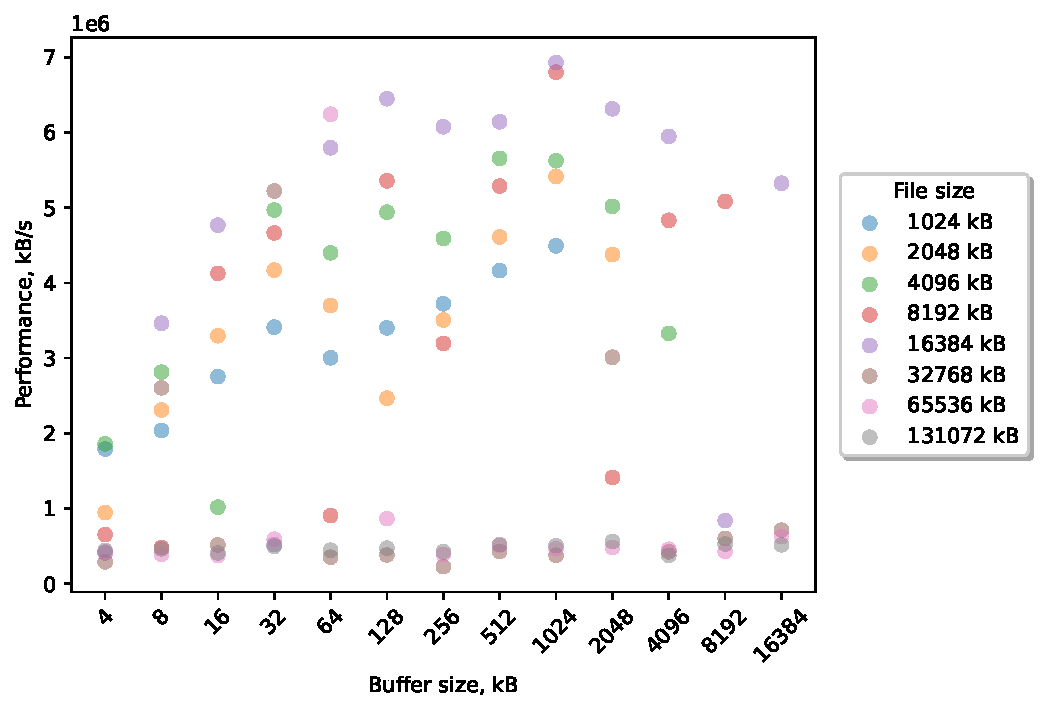
\includegraphics[width=1.0\textwidth]{figures.nosync/benchmarking/old/gcsf/Read.pdf}
% 	\end{center}
% 	\caption{IOZone output for GCSF Forward Read}
% \end{figure}

% \begin{figure}[!htb]
% 	\label{fig:app_begcsf_ffs_write}
% 	\begin{center}
% 		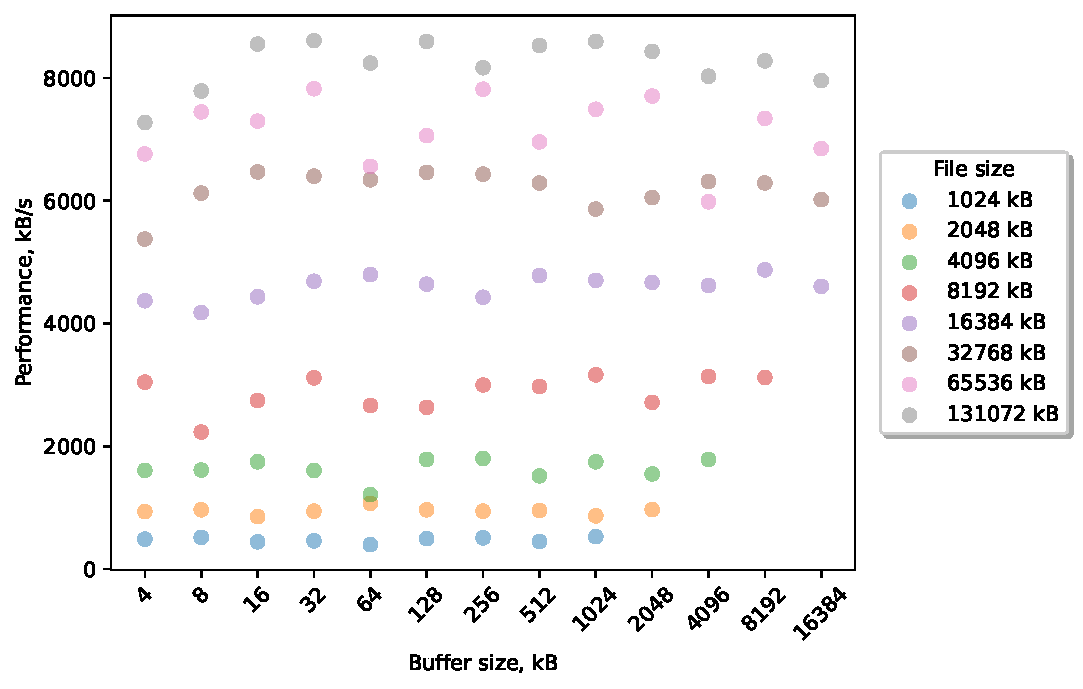
\includegraphics[width=1.0\textwidth]{figures.nosync/benchmarking/old/gcsf/Write.pdf}
% 	\end{center}
% 	\caption{IOZone output for GCSF Forward Write}
% \end{figure}

% \begin{figure}[!htb]
% 	\label{fig:app_bencgcsffs_re_read}
% 	\begin{center}
% 		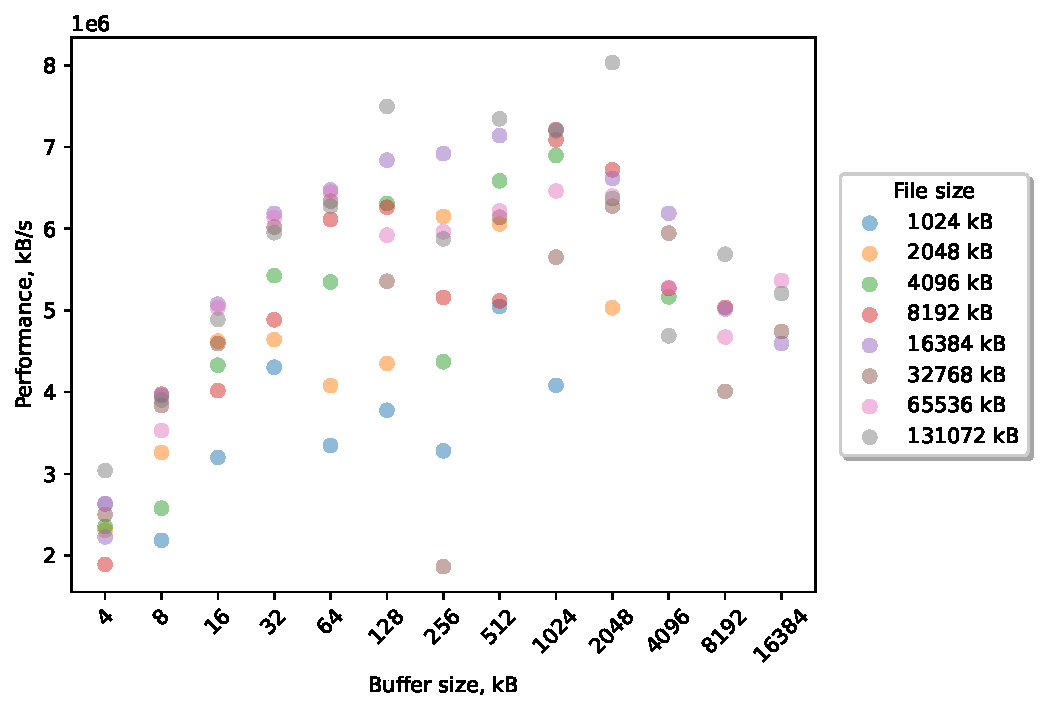
\includegraphics[width=1.0\textwidth]{figures.nosync/benchmarking/old/gcsf/Re-Read.pdf}
% 	\end{center}
% 	\caption{IOZone output for GCSF \mbox{Re-Read}}
% \end{figure}

% \begin{figure}[!htb]
% 	\label{fig:app_benchgcsfs_re_write}
% 	\begin{center}
% 		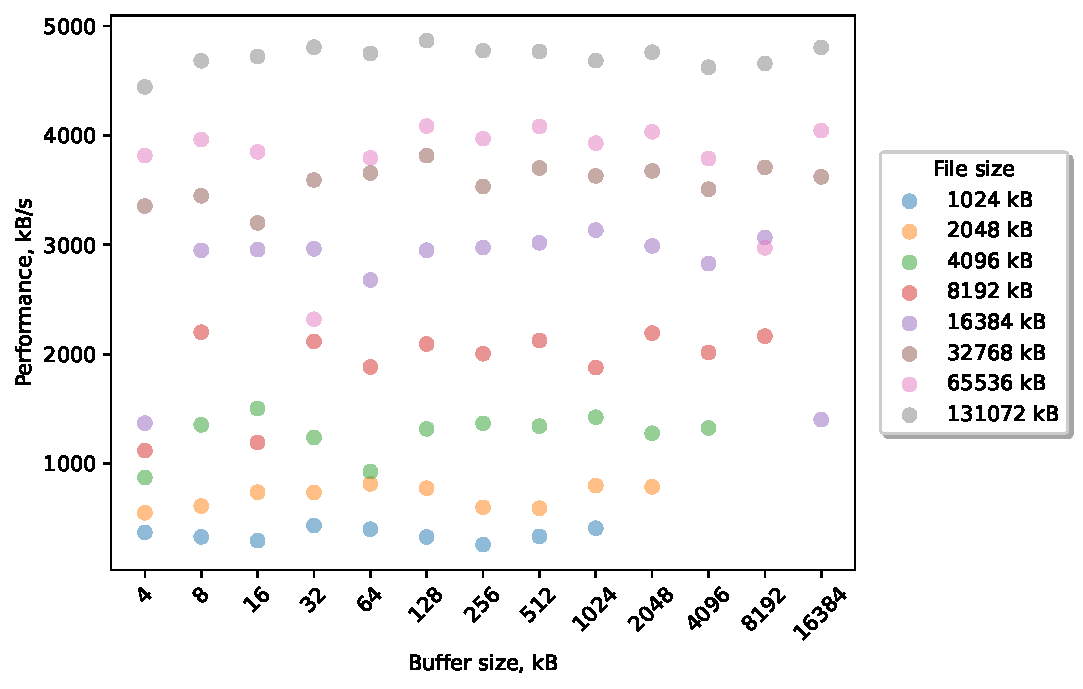
\includegraphics[width=1.0\textwidth]{figures.nosync/benchmarking/old/gcsf/Re-Write.pdf}
% 	\end{center}
% 	\caption{IOZone output for GCSF \mbox{Re-Write}}
% \end{figure}

% \begin{figure}[!htb]
% 	\label{fig:app_benchgcsfs_rnd_read}
% 	\begin{center}
% 		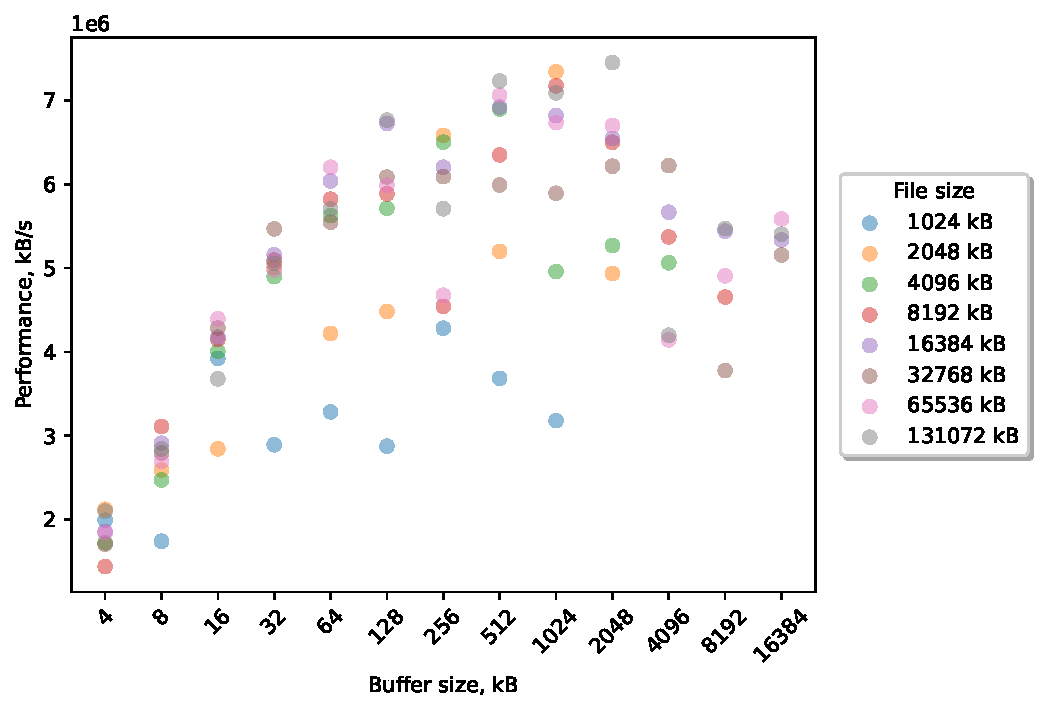
\includegraphics[width=1.0\textwidth]{figures.nosync/benchmarking/old/gcsf/Random read.pdf}
% 	\end{center}
% 	\caption{IOZone output for GCSF Random read}
% \end{figure}

% \begin{figure}[!htb]
% 	\label{fig:app_bench_gcsf_rnd_write}
% 	\begin{center}
% 		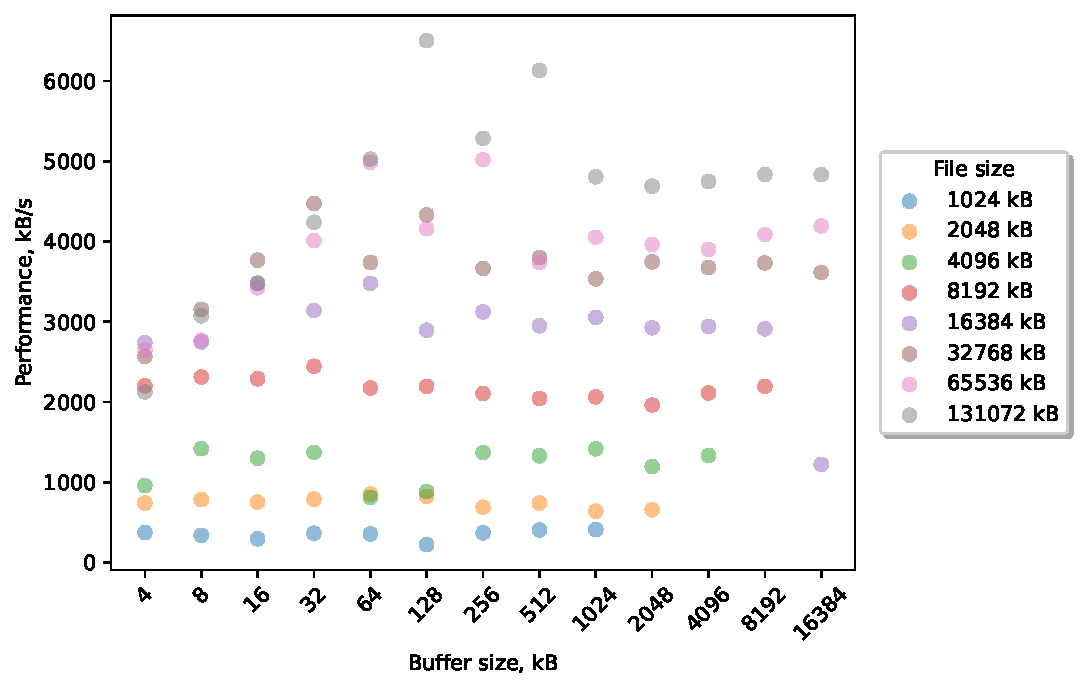
\includegraphics[width=1.0\textwidth]{figures.nosync/benchmarking/old/gcsf/Random write.pdf}
% 	\end{center}
% 	\caption{IOZone output for GCSF Random write}
% \end{figure}

\newpage

\section{Fejk FFS}

\begin{table}[!ht]
	\begin{center}
		\caption{IOZone result for the Read test on FFFS in kilobytes per second}
		\resizebox{\textwidth}{!}{\begin{tabular}{| r | r | r | r | r | r | r | r | r | r | r | r | r | r | }
			
			\hline
			{} & \multicolumn{13}{c |}{Buffer size (kB)} \\
			\textbf{File size (kB)}   & \multicolumn{1}{c |}{4} & \multicolumn{1}{c |}{8} & \multicolumn{1}{c |}{16} & \multicolumn{1}{c |}{32} & \multicolumn{1}{c |}{64} & \multicolumn{1}{c |}{128} & \multicolumn{1}{c |}{256} & \multicolumn{1}{c |}{512} & \multicolumn{1}{c |}{1024} & \multicolumn{1}{c |}{2048} & \multicolumn{1}{c |}{4096} & \multicolumn{1}{c |}{8192} & \multicolumn{1}{c |}{16384}\\
			\hline
			\hline
			\textbf{1024}  & 1605111 & 2472911 & 889631 & 2715230 & 3618930 & 3001782 & 1032244 & 2578312 & 2467229 & {} & {} & {} & {}\\
			\textbf{2048}  & 1921339 & 1930406 & 2194777 & 2821176 & 3200654 & 4130162 & 4154130 & 2649737 & 5032754 & 3286370 & {} & {} & {}\\
			\textbf{4096}  & 2426601 & 2784507 & 3271230 & 3574071 & 3670280 & 5542240 & 4386193 & 3771811 & 3995498 & 4763181 & 4000150 & {} & {}\\
			\textbf{8192}  & 2895693 & 3535750 & 4173008 & 5378957 & 4899570 & 4548665 & 5914094 & 6558696 & 4271046 & 4104220 & 5475825 & 5888754 & {}\\
			\textbf{16384}  & 3094244 & 4152032 & 4908602 & 3512941 & 6234299 & 5855539 & 6313919 & 7272051 & 6212881 & 7111751 & 5507336 & 5387732 & 5486670\\
			\textbf{32768}  & 2848900 & 3537882 & 4681672 & 6104381 & 6554760 & 5933093 & 6802626 & 6375072 & 6339199 & 6146697 & 6030191 & 5591994 & 5440583\\
			\textbf{65536}  & 70116 & 3562495 & 5159913 & 5999237 & 7335592 & 7026566 & 7648924 & 6445904 & 77043 & 129764 & 5783761 & 5526649 & 4978066\\
			\textbf{131072}  & 394463 & 2034461 & 454646 & 6311863 & 3782086 & 280028 & 7525973 & 6890568 & 75477 & 59220 & 2674224 & 238745 & 657556\\
			\textbf{262144}  & 65486 & 75529 & 77854 & 97658 & 79916 & 72736 & 76276 & 71780 & 106689 & 72269 & 72176 & 79924 & 126614\\


			\hline

		\end{tabular}}
		\label{tbl:data_fejk-ffs_read}
	\end{center}
\end{table}
	
\begin{table}[!ht]
	\begin{center}
		\caption{IOZone result for the Write test on FFFS in kilobytes per second}
		\resizebox{\textwidth}{!}{\begin{tabular}{| r | r | r | r | r | r | r | r | r | r | r | r | r | r | }
			
			\hline
			{} & \multicolumn{13}{c |}{Buffer size (kB)} \\
			\textbf{File size (kB)}   & \multicolumn{1}{c |}{4} & \multicolumn{1}{c |}{8} & \multicolumn{1}{c |}{16} & \multicolumn{1}{c |}{32} & \multicolumn{1}{c |}{64} & \multicolumn{1}{c |}{128} & \multicolumn{1}{c |}{256} & \multicolumn{1}{c |}{512} & \multicolumn{1}{c |}{1024} & \multicolumn{1}{c |}{2048} & \multicolumn{1}{c |}{4096} & \multicolumn{1}{c |}{8192} & \multicolumn{1}{c |}{16384}\\
			\hline
			\hline
			\textbf{1024}  & 5193 & 5287 & 4303 & 5160 & 5076 & 5282 & 27847 & 5736 & 5086 & {} & {} & {} & {}\\
			\textbf{2048}  & 4807 & 5335 & 4665 & 6305 & 6258 & 5920 & 6228 & 6453 & 5811 & 6301 & {} & {} & {}\\
			\textbf{4096}  & 5767 & 5943 & 5979 & 5807 & 6265 & 6320 & 3784 & 6770 & 5759 & 6188 & 6844 & {} & {}\\
			\textbf{8192}  & 5504 & 6464 & 6702 & 6783 & 6175 & 6015 & 5288 & 6874 & 98659 & 101980 & 7043 & 6738 & {}\\
			\textbf{16384}  & 6430 & 6955 & 7463 & 7442 & 6794 & 7637 & 7667 & 7628 & 7337 & 101677 & 7553 & 7824 & 7735\\
			\textbf{32768}  & 7232 & 7656 & 7808 & 7859 & 8075 & 8142 & 8075 & 8062 & 8161 & 7896 & 8229 & 117474 & 8377\\
			\textbf{65536}  & 7370 & 7246 & 7273 & 7350 & 7530 & 7664 & 7658 & 8170 & 6959 & 7196 & 7192 & 7019 & 6735\\
			\textbf{131072}  & 7160 & 6974 & 6961 & 7229 & 7593 & 7217 & 7901 & 8196 & 8116 & 5763 & 7398 & 5990 & 8025\\
			\textbf{262144}  & 7167 & 7419 & 7937 & 7545 & 8435 & 8520 & 8030 & 7742 & 3996 & 7468 & 7601 & 8066 & 7891\\
			\textbf{524288}  & 7578 & 7967 & 8161 & 82 & 8189 & 8494 & 8454 & 8327 & 8466 & 8501 & 8370 & 8308 & 5935\\


			\hline

		\end{tabular}}
		\label{tbl:data_fejk-ffs_write}
	\end{center}
\end{table}
	
\begin{table}[!ht]
	\begin{center}
		\caption{IOZone result for the Re-Read test on FFFS in kilobytes per second}
		\resizebox{\textwidth}{!}{\begin{tabular}{| r | r | r | r | r | r | r | r | r | r | r | r | r | r | }
			
			\hline
			{} & \multicolumn{13}{c |}{Buffer size (kB)} \\
			\textbf{File size (kB)}   & \multicolumn{1}{c |}{4} & \multicolumn{1}{c |}{8} & \multicolumn{1}{c |}{16} & \multicolumn{1}{c |}{32} & \multicolumn{1}{c |}{64} & \multicolumn{1}{c |}{128} & \multicolumn{1}{c |}{256} & \multicolumn{1}{c |}{512} & \multicolumn{1}{c |}{1024} & \multicolumn{1}{c |}{2048} & \multicolumn{1}{c |}{4096} & \multicolumn{1}{c |}{8192} & \multicolumn{1}{c |}{16384}\\
			\hline
			\hline
			\textbf{1024}  & 1984913 & 2820430 & 2353657 & 4674510 & 4232305 & 3198502 & 1920993 & 4943530 & 3142339 & {} & {} & {} & {}\\
			\textbf{2048}  & 2107025 & 3011047 & 2367151 & 3915540 & 4633675 & 5209791 & 5119743 & 4663865 & 4829046 & 3736694 & {} & {} & {}\\
			\textbf{4096}  & 3075079 & 3614679 & 4462528 & 4302706 & 5971855 & 6503078 & 4906002 & 6471234 & 4132949 & 5184332 & 3442303 & {} & {}\\
			\textbf{8192}  & 2826843 & 4114541 & 4678737 & 5261179 & 4158362 & 6182248 & 5094251 & 5357152 & 6537482 & 5382328 & 5756551 & 5915112 & {}\\
			\textbf{16384}  & 3115426 & 4517212 & 5147601 & 6343059 & 6609036 & 6262707 & 6753222 & 7984318 & 6787239 & 7246745 & 5728625 & 5310703 & 5452279\\
			\textbf{32768}  & 2786858 & 3742299 & 5009656 & 7004755 & 7299786 & 7123475 & 7777741 & 6994062 & 6752162 & 7039557 & 6382473 & 5967613 & 5664360\\
			\textbf{65536}  & 2205856 & 4396090 & 5428742 & 6393876 & 6889031 & 6089074 & 7811071 & 6860318 & 7461842 & 6801920 & 6440769 & 5750246 & 4823451\\
			\textbf{131072}  & 3287977 & 3847707 & 5198793 & 6348527 & 6951999 & 8443258 & 7909267 & 7114111 & 7388515 & 5298401 & 3139222 & 5802490 & 6479087\\
			\textbf{262144}  & 2974653 & 4452026 & 5376537 & 6145825 & 7115944 & 7217446 & 7116911 & 6533364 & 6027138 & 6506108 & 5360469 & 5598732 & 5819467\\


			\hline

		\end{tabular}}
		\label{tbl:data_fejk-ffs_re-read}
	\end{center}
\end{table}
	
\begin{table}[!ht]
	\begin{center}
		\caption{IOZone result for the Re-Write test on FFFS in kilobytes per second}
		\resizebox{\textwidth}{!}{\begin{tabular}{| r | r | r | r | r | r | r | r | r | r | r | r | r | r | }
			
			\hline
			{} & \multicolumn{13}{c |}{Buffer size (kB)} \\
			\textbf{File size (kB)}   & \multicolumn{1}{c |}{4} & \multicolumn{1}{c |}{8} & \multicolumn{1}{c |}{16} & \multicolumn{1}{c |}{32} & \multicolumn{1}{c |}{64} & \multicolumn{1}{c |}{128} & \multicolumn{1}{c |}{256} & \multicolumn{1}{c |}{512} & \multicolumn{1}{c |}{1024} & \multicolumn{1}{c |}{2048} & \multicolumn{1}{c |}{4096} & \multicolumn{1}{c |}{8192} & \multicolumn{1}{c |}{16384}\\
			\hline
			\hline
			\textbf{1024}  & 4574 & 4975 & 1566 & 5157 & 4391 & 4913 & 3380 & 27982 & 5001 & {} & {} & {} & {}\\
			\textbf{2048}  & 3371 & 4654 & 5206 & 4614 & 5631 & 5635 & 5680 & 31266 & 5577 & 5685 & {} & {} & {}\\
			\textbf{4096}  & 5548 & 5728 & 5588 & 5188 & 5330 & 5148 & 5077 & 5928 & 5449 & 4753 & 5515 & {} & {}\\
			\textbf{8192}  & 5296 & 5167 & 5574 & 5177 & 5002 & 5540 & 5362 & 5527 & 5913 & 5893 & 5485 & 4895 & {}\\
			\textbf{16384}  & 5933 & 5866 & 6309 & 6263 & 5714 & 6230 & 6215 & 6563 & 6454 & 6412 & 5640 & 25482 & 6565\\
			\textbf{32768}  & 6314 & 6369 & 6575 & 6687 & 6841 & 6852 & 6824 & 6819 & 6889 & 6768 & 6782 & 6699 & 6885\\
			\textbf{65536}  & 5933 & 6327 & 5753 & 6290 & 6514 & 5615 & 6329 & 6632 & 5962 & 5815 & 5749 & 5935 & 25761\\
			\textbf{131072}  & 5885 & 5619 & 6099 & 6598 & 6601 & 5990 & 6717 & 6763 & 5816 & 4048 & 6124 & 4737 & 6436\\
			\textbf{262144}  & 5769 & 6203 & 6474 & 6722 & 6879 & 6865 & 6565 & 6140 & 6177 & 6033 & 6164 & 6586 & 6653\\


			\hline

		\end{tabular}}
		\label{tbl:data_fejk-ffs_re-write}
	\end{center}
\end{table}
	
\begin{table}[!ht]
	\begin{center}
		\caption{IOZone result for the Random read test on FFFS in kilobytes per second}
		\resizebox{\textwidth}{!}{\begin{tabular}{| r | r | r | r | r | r | r | r | r | r | r | r | r | r | }
			
			\hline
			{} & \multicolumn{13}{c |}{Buffer size (kB)} \\
			\textbf{File size (kB)}   & \multicolumn{1}{c |}{4} & \multicolumn{1}{c |}{8} & \multicolumn{1}{c |}{16} & \multicolumn{1}{c |}{32} & \multicolumn{1}{c |}{64} & \multicolumn{1}{c |}{128} & \multicolumn{1}{c |}{256} & \multicolumn{1}{c |}{512} & \multicolumn{1}{c |}{1024} & \multicolumn{1}{c |}{2048} & \multicolumn{1}{c |}{4096} & \multicolumn{1}{c |}{8192} & \multicolumn{1}{c |}{16384}\\
			\hline
			\hline
			\textbf{1024}  & 1438461 & 2474336 & 3335105 & 4339202 & 4574926 & 3594699 & 1662264 & 4415030 & 3390391 & {} & {} & {} & {}\\
			\textbf{2048}  & 1639674 & 2531808 & 2980747 & 3071337 & 4971585 & 5626082 & 5235193 & 4240255 & 3864455 & 4591569 & {} & {} & {}\\
			\textbf{4096}  & 2333965 & 2898672 & 4076076 & 4214051 & 3641495 & 6716643 & 3128843 & 6022095 & 4428023 & 4935601 & 5551194 & {} & {}\\
			\textbf{8192}  & 2217071 & 1882745 & 4242044 & 6006101 & 3655755 & 6054786 & 6947247 & 6912307 & 6339662 & 5785631 & 5789530 & 5583494 & {}\\
			\textbf{16384}  & 2235520 & 2613523 & 4010753 & 5637917 & 5897753 & 5362924 & 6542963 & 7922644 & 6671272 & 7117644 & 4702688 & 5233056 & 5189585\\
			\textbf{32768}  & 1953956 & 2985674 & 4118168 & 6358850 & 7157605 & 6732647 & 7552086 & 7015482 & 6541968 & 7126430 & 6545707 & 5985025 & 5650853\\
			\textbf{65536}  & 1320279 & 3522910 & 4420978 & 5494832 & 6317898 & 6091233 & 7578280 & 6635907 & 7317626 & 6684480 & 6613236 & 5663404 & 4218907\\
			\textbf{131072}  & 2179297 & 3011967 & 4211016 & 5669935 & 6324062 & 7899720 & 7685258 & 6951208 & 7292757 & 5564284 & 2867974 & 5863448 & 6536945\\
			\textbf{262144}  & 2105727 & 3331986 & 4265958 & 5398262 & 6599796 & 7121152 & 6889437 & 6293359 & 6270783 & 5819868 & 5256751 & 5823875 & 5831010\\


			\hline

		\end{tabular}}
		\label{tbl:data_fejk-ffs_random_read}
	\end{center}
\end{table}
	
\begin{table}[!ht]
	\begin{center}
		\caption{IOZone result for the Random write test on FFFS in kilobytes per second}
		\resizebox{\textwidth}{!}{\begin{tabular}{| r | r | r | r | r | r | r | r | r | r | r | r | r | r | }
			
			\hline
			{} & \multicolumn{13}{c |}{Buffer size (kB)} \\
			\textbf{File size (kB)}   & \multicolumn{1}{c |}{4} & \multicolumn{1}{c |}{8} & \multicolumn{1}{c |}{16} & \multicolumn{1}{c |}{32} & \multicolumn{1}{c |}{64} & \multicolumn{1}{c |}{128} & \multicolumn{1}{c |}{256} & \multicolumn{1}{c |}{512} & \multicolumn{1}{c |}{1024} & \multicolumn{1}{c |}{2048} & \multicolumn{1}{c |}{4096} & \multicolumn{1}{c |}{8192} & \multicolumn{1}{c |}{16384}\\
			\hline
			\hline
			\textbf{1024}  & 4619 & 4008 & 2880 & 4530 & 4425 & 4764 & 3097 & 5879 & 4465 & {} & {} & {} & {}\\
			\textbf{2048}  & 4620 & 4691 & 5179 & 5665 & 5728 & 5660 & 4573 & 5554 & 5775 & 5519 & {} & {} & {}\\
			\textbf{4096}  & 5284 & 5681 & 5333 & 5194 & 5488 & 5822 & 5854 & 6127 & 37216 & 5145 & 5738 & {} & {}\\
			\textbf{8192}  & 5442 & 4747 & 5737 & 5386 & 5800 & 5088 & 5881 & 5811 & 5414 & 5708 & 4852 & 5635 & {}\\
			\textbf{16384}  & 5553 & 6011 & 6191 & 6267 & 6188 & 5654 & 6348 & 6585 & 6428 & 6509 & 5831 & 6558 & 6496\\
			\textbf{32768}  & 6253 & 6238 & 6434 & 6511 & 6810 & 6829 & 6984 & 6800 & 6877 & 6801 & 6853 & 6875 & 6857\\
			\textbf{65536}  & 4967 & 6318 & 5379 & 5753 & 6616 & 6361 & 6528 & 6611 & 5854 & 5900 & 5980 & 6472 & 5881\\
			\textbf{131072}  & 5754 & 5611 & 6114 & 6317 & 6102 & 6407 & 6469 & 6662 & 4629 & 4861 & 5661 & 5536 & 6443\\
			\textbf{262144}  & 5741 & 6259 & 6439 & 6689 & 6907 & 6427 & 6463 & 6100 & 6309 & 5998 & 6035 & 6849 & 6857\\


			\hline

		\end{tabular}}
		\label{tbl:data_fejk-ffs_random_write}
	\end{center}
\end{table}
	

\FloatBarrier
% \begin{figure}[!htb]
% 	\label{fig:app_bencfh_ffs_read}
% 	\begin{center}
% 		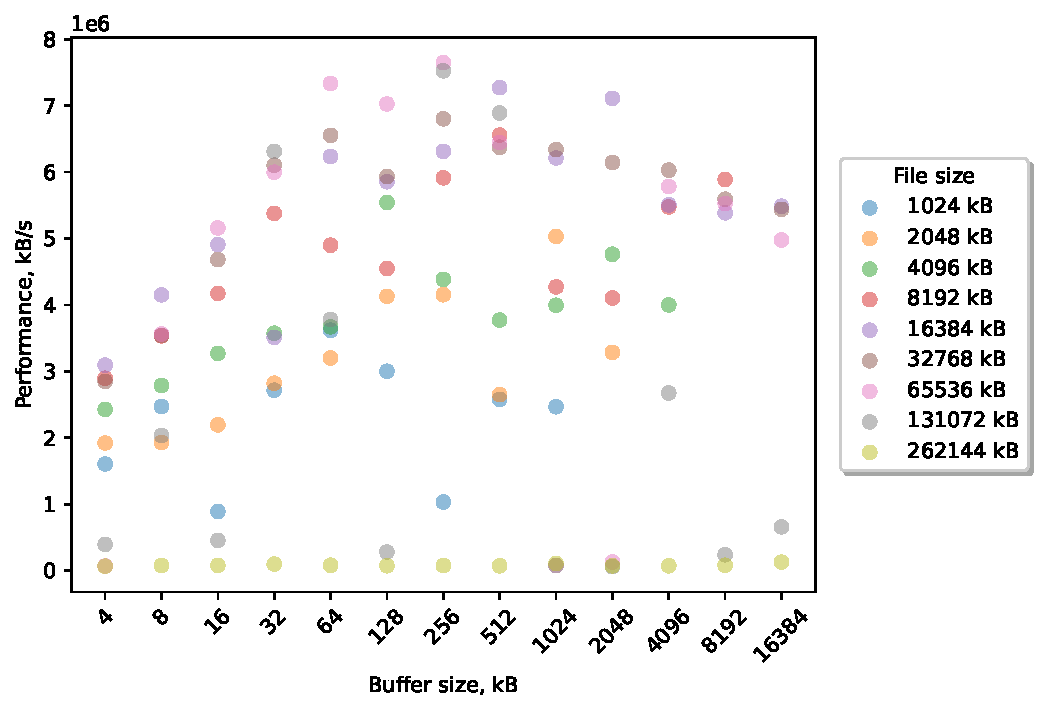
\includegraphics[width=1.0\textwidth]{figures.nosync/benchmarking/old/fejk-ffs/Read.pdf}
% 	\end{center}
% 	\caption{IOZone output for Fejk FFS Forward Read}
% \end{figure}

% \begin{figure}[!htb]
% 	\label{fig:app_benchf_ffs_write}
% 	\begin{center}
% 		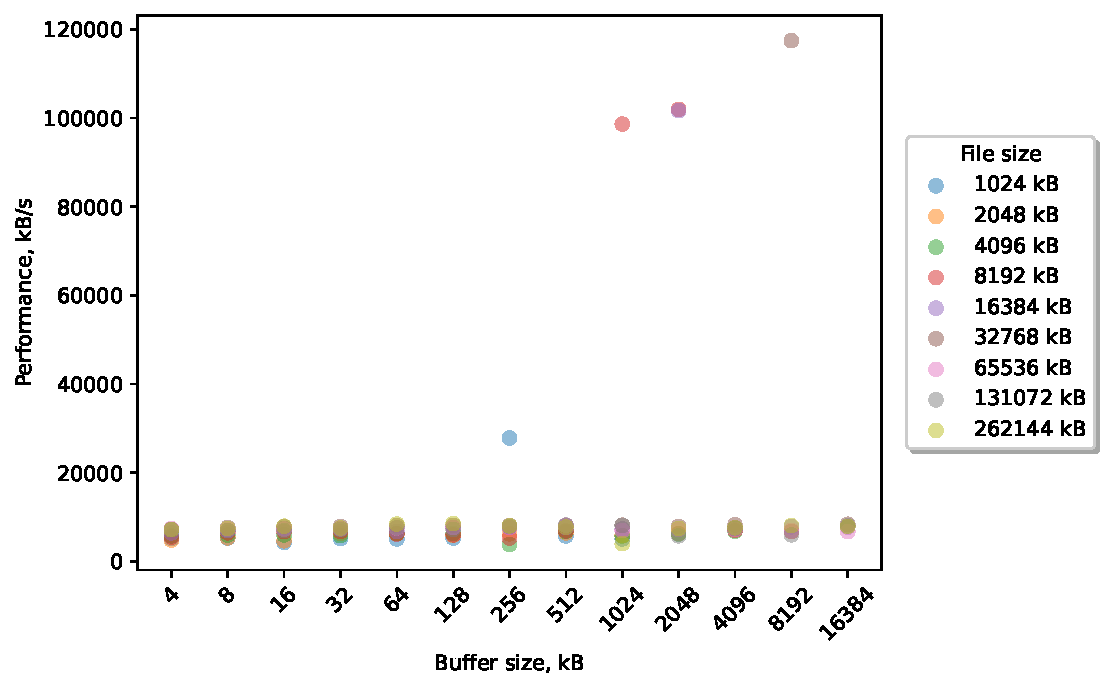
\includegraphics[width=1.0\textwidth]{figures.nosync/benchmarking/old/fejk-ffs/Write.pdf}
% 	\end{center}
% 	\caption{IOZone output for Fejk FFS Forward Write}
% \end{figure}

% \begin{figure}[!htb]
% 	\label{fig:app_bench_fffs_re_read}
% 	\begin{center}
% 		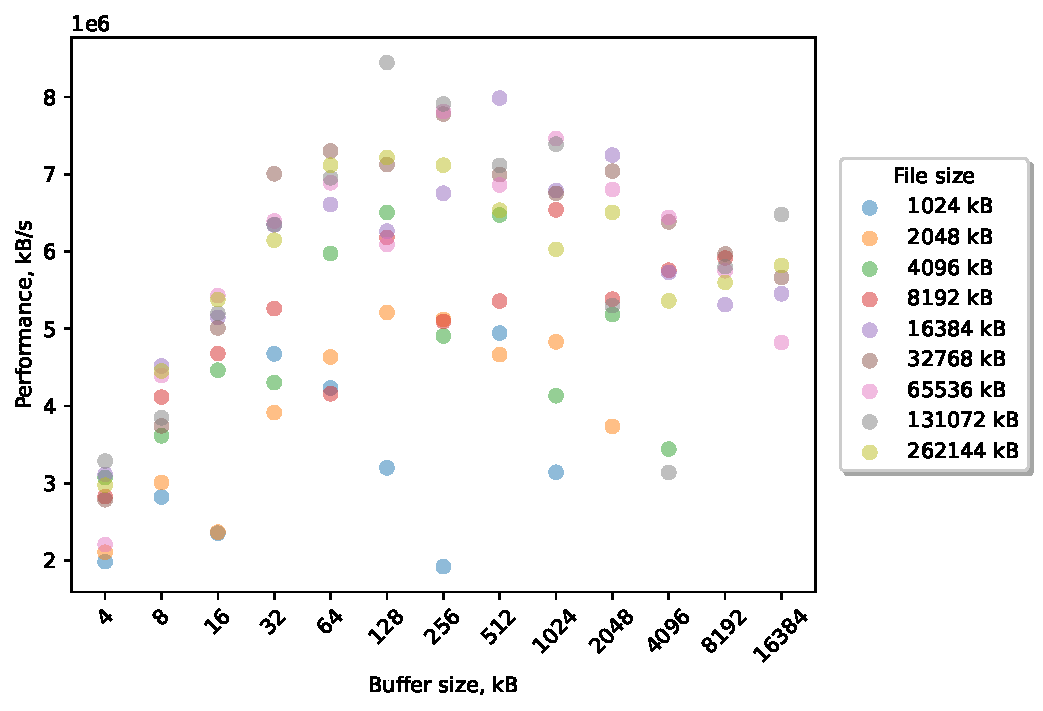
\includegraphics[width=1.0\textwidth]{figures.nosync/benchmarking/old/fejk-ffs/Re-Read.pdf}
% 	\end{center}
% 	\caption{IOZone output for Fejk FFS \mbox{Re-Read}}
% \end{figure}

% \begin{figure}[!htb]
% 	\label{fig:app_bench_fffs_re_write}
% 	\begin{center}
% 		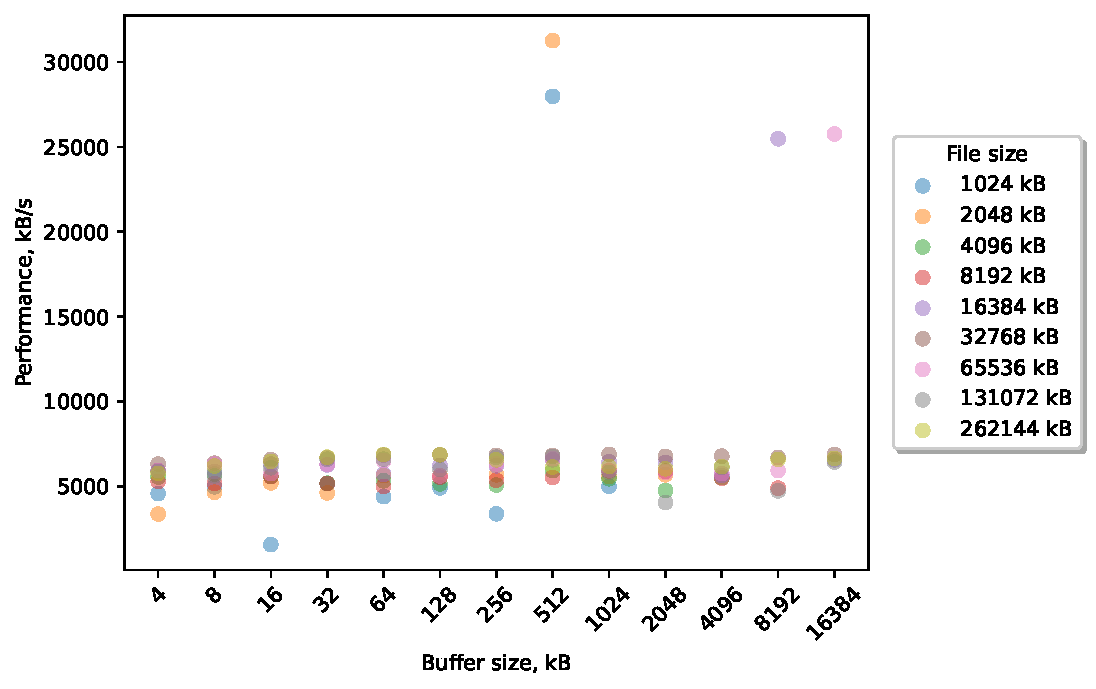
\includegraphics[width=1.0\textwidth]{figures.nosync/benchmarking/old/fejk-ffs/Re-Write.pdf}
% 	\end{center}
% 	\caption{IOZone output for Fejk FFS \mbox{Re-Write}}
% \end{figure}

% \begin{figure}[!htb]
% 	\label{fig:app_bench_fffs_rnd_read}
% 	\begin{center}
% 		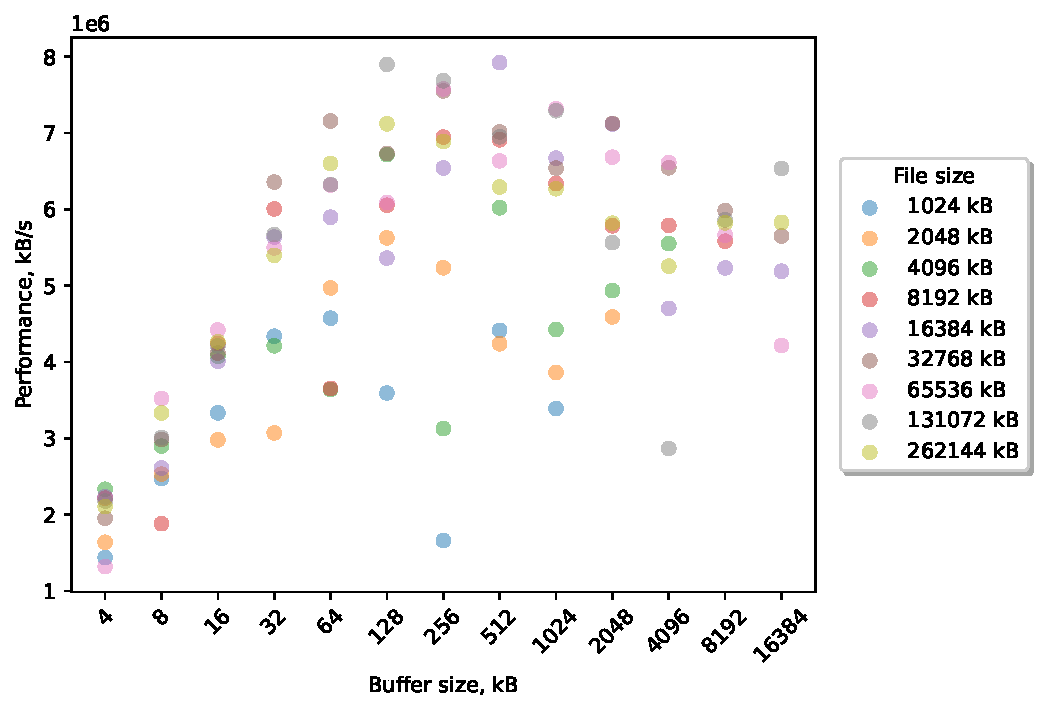
\includegraphics[width=1.0\textwidth]{figures.nosync/benchmarking/old/fejk-ffs/Random read.pdf}
% 	\end{center}
% 	\caption{IOZone output for Fejk FFS Random read}
% \end{figure}

% \begin{figure}[!htb]
% 	\label{fig:app_bench_ffsf_rnd_write}
% 	\begin{center}
% 		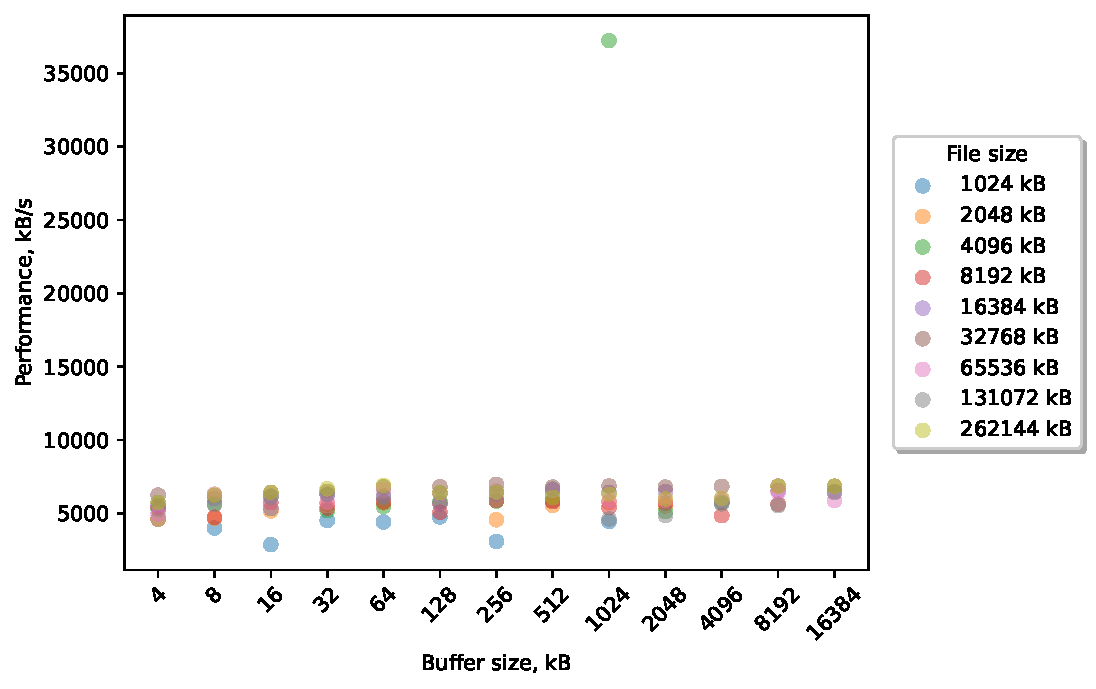
\includegraphics[width=1.0\textwidth]{figures.nosync/benchmarking/old/fejk-ffs/Random write.pdf}
% 	\end{center}
% 	\caption{IOZone output for Fejk FFS Random write}
% \end{figure}
\newpage

\section{APFS}

\begin{table}[!ht]
	\begin{center}
		\caption{IOZone result for the Read test on APFS in kilobytes per second}
		\resizebox{\textwidth}{!}{\begin{tabular}{| r | r | r | r | r | r | r | r | r | r | r | r | r | r | }
			
			\hline
			{} & \multicolumn{13}{c |}{Buffer size (kB)} \\
			\textbf{File size (kB)}   & \multicolumn{1}{c |}{4} & \multicolumn{1}{c |}{8} & \multicolumn{1}{c |}{16} & \multicolumn{1}{c |}{32} & \multicolumn{1}{c |}{64} & \multicolumn{1}{c |}{128} & \multicolumn{1}{c |}{256} & \multicolumn{1}{c |}{512} & \multicolumn{1}{c |}{1024} & \multicolumn{1}{c |}{2048} & \multicolumn{1}{c |}{4096} & \multicolumn{1}{c |}{8192} & \multicolumn{1}{c |}{16384}\\
			\hline
			\hline
			\textbf{1024}  & 538364 & 3908759 & 4488860 & 6128613 & 5251818 & 5660167 & 6402699 & 7420395 & 8474583 & {} & {} & {} & {}\\
			\textbf{2048}  & 2582813 & 3379461 & 4172290 & 5644567 & 5184636 & 6583305 & 5280246 & 6603549 & 8159088 & 7393606 & {} & {} & {}\\
			\textbf{4096}  & 2523925 & 3846119 & 4591331 & 5918366 & 6459069 & 6225028 & 6471234 & 5728903 & 7085049 & 6198078 & 5558378 & {} & {}\\
			\textbf{8192}  & 2689438 & 3653812 & 4902367 & 5603526 & 6081578 & 6310553 & 6720329 & 6809564 & 7067279 & 7154097 & 5422249 & 5776876 & {}\\
			\textbf{16384}  & 2675387 & 3779365 & 5457909 & 6347747 & 7440550 & 6818216 & 7702417 & 3990259 & 6054683 & 6367155 & 6698584 & 5477922 & 5027467\\
			\textbf{32768}  & 2654604 & 4438267 & 5507073 & 6566975 & 4920870 & 6247564 & 6546954 & 6621073 & 5274791 & 7583338 & 2896268 & 5498920 & 5641806\\
			\textbf{65536}  & 2574587 & 4011012 & 4825568 & 5732617 & 6554261 & 6607037 & 6608467 & 6864601 & 6640556 & 6608467 & 4768972 & 5492416 & 5470445\\
			\textbf{131072}  & 2665860 & 3968043 & 5421344 & 5545873 & 5938696 & 6221082 & 6147894 & 6289118 & 6388735 & 2839445 & 3350171 & 5215562 & 4865147\\
			\textbf{262144}  & 2385943 & 2904121 & 4293712 & 5289093 & 4596201 & 6348519 & 6435168 & 7442619 & 7397503 & 7744086 & 6419575 & 5641535 & 3369068\\


			\hline

		\end{tabular}}
		\label{tbl:data_local_read}
	\end{center}
\end{table}
	
\begin{table}[!ht]
	\begin{center}
		\caption{IOZone result for the Write test on APFS in kilobytes per second}
		\resizebox{\textwidth}{!}{\begin{tabular}{| r | r | r | r | r | r | r | r | r | r | r | r | r | r | }
			
			\hline
			{} & \multicolumn{13}{c |}{Buffer size (kB)} \\
			\textbf{File size (kB)}   & \multicolumn{1}{c |}{4} & \multicolumn{1}{c |}{8} & \multicolumn{1}{c |}{16} & \multicolumn{1}{c |}{32} & \multicolumn{1}{c |}{64} & \multicolumn{1}{c |}{128} & \multicolumn{1}{c |}{256} & \multicolumn{1}{c |}{512} & \multicolumn{1}{c |}{1024} & \multicolumn{1}{c |}{2048} & \multicolumn{1}{c |}{4096} & \multicolumn{1}{c |}{8192} & \multicolumn{1}{c |}{16384}\\
			\hline
			\hline
			\textbf{1024}  & 186358 & 335392 & 512232 & 827258 & 699870 & 1032244 & 1273788 & 1477555 & 873705 & {} & {} & {} & {}\\
			\textbf{2048}  & 229598 & 236085 & 291779 & 397593 & 892849 & 514465 & 513420 & 574009 & 1394966 & 1341170 & {} & {} & {}\\
			\textbf{4096}  & 190955 & 306150 & 512697 & 562558 & 593887 & 959243 & 806157 & 867415 & 754866 & 642314 & 1117622 & {} & {}\\
			\textbf{8192}  & 169441 & 255864 & 357293 & 401784 & 651754 & 675577 & 650779 & 675976 & 564729 & 633023 & 708889 & 752384 & {}\\
			\textbf{16384}  & 229954 & 310425 & 353652 & 491394 & 722178 & 716747 & 601890 & 639573 & 775984 & 708683 & 579081 & 698945 & 784336\\
			\textbf{32768}  & 201952 & 299576 & 431731 & 562454 & 584277 & 593696 & 609775 & 421778 & 769363 & 662034 & 427841 & 483047 & 741123\\
			\textbf{65536}  & 205960 & 323049 & 351173 & 451792 & 416014 & 504320 & 495422 & 632520 & 336679 & 473751 & 501468 & 662240 & 523098\\
			\textbf{131072}  & 210777 & 300665 & 358868 & 352807 & 399321 & 527975 & 431966 & 419926 & 413309 & 349982 & 282681 & 307020 & 224134\\
			\textbf{262144}  & 213134 & 286667 & 418873 & 410737 & 231669 & 474854 & 322547 & 305477 & 446954 & 702936 & 283134 & 563923 & 396791\\


			\hline

		\end{tabular}}
		\label{tbl:data_local_write}
	\end{center}
\end{table}
	
\begin{table}[!ht]
	\begin{center}
		\caption{IOZone result for the Re-Read test on APFS in kilobytes per second}
		\resizebox{\textwidth}{!}{\begin{tabular}{| r | r | r | r | r | r | r | r | r | r | r | r | r | r | }
			
			\hline
			{} & \multicolumn{13}{c |}{Buffer size (kB)} \\
			\textbf{File size (kB)}   & \multicolumn{1}{c |}{4} & \multicolumn{1}{c |}{8} & \multicolumn{1}{c |}{16} & \multicolumn{1}{c |}{32} & \multicolumn{1}{c |}{64} & \multicolumn{1}{c |}{128} & \multicolumn{1}{c |}{256} & \multicolumn{1}{c |}{512} & \multicolumn{1}{c |}{1024} & \multicolumn{1}{c |}{2048} & \multicolumn{1}{c |}{4096} & \multicolumn{1}{c |}{8192} & \multicolumn{1}{c |}{16384}\\
			\hline
			\hline
			\textbf{1024}  & 2942149 & 4300102 & 4898425 & 7420395 & 8000971 & 6918376 & 8970167 & 8199542 & 10662628 & {} & {} & {} & {}\\
			\textbf{2048}  & 2892423 & 4038890 & 4911886 & 9101380 & 6967792 & 8059569 & 4284671 & 8464610 & 9898453 & 10660056 & {} & {} & {}\\
			\textbf{4096}  & 2603876 & 3991785 & 4853336 & 6330545 & 7380284 & 6669706 & 7355007 & 7135072 & 7515892 & 6625976 & 5744227 & {} & {}\\
			\textbf{8192}  & 2578436 & 3948121 & 5047109 & 6118398 & 6627005 & 6855760 & 7205103 & 7386322 & 7474698 & 8152152 & 4955393 & 5013234 & {}\\
			\textbf{16384}  & 2666252 & 3689278 & 5628220 & 6660280 & 7736235 & 7050461 & 8087683 & 3954666 & 5923170 & 6405137 & 5624535 & 5472251 & 4733787\\
			\textbf{32768}  & 2459325 & 4444294 & 5092820 & 6114429 & 5524116 & 6207215 & 6885441 & 6739910 & 5866989 & 6999048 & 2186853 & 5164391 & 5674182\\
			\textbf{65536}  & 2609539 & 3811988 & 4921646 & 5591403 & 6577945 & 6843750 & 6577315 & 7125655 & 7737415 & 6903565 & 4937914 & 5074468 & 5140421\\
			\textbf{131072}  & 2795139 & 3709708 & 5510463 & 5775607 & 6114321 & 6257620 & 5947047 & 6486732 & 5777367 & 2253302 & 2813722 & 4947994 & 4669283\\
			\textbf{262144}  & 2259139 & 3316468 & 3623921 & 4864863 & 5380721 & 6522434 & 7086865 & 7440101 & 6565902 & 6814965 & 6387391 & 5202306 & 4402011\\


			\hline

		\end{tabular}}
		\label{tbl:data_local_re-read}
	\end{center}
\end{table}
	
\begin{table}[!ht]
	\begin{center}
		\caption{IOZone result for the Re-Write test on APFS in kilobytes per second}
		\resizebox{\textwidth}{!}{\begin{tabular}{| r | r | r | r | r | r | r | r | r | r | r | r | r | r | }
			
			\hline
			{} & \multicolumn{13}{c |}{Buffer size (kB)} \\
			\textbf{File size (kB)}   & \multicolumn{1}{c |}{4} & \multicolumn{1}{c |}{8} & \multicolumn{1}{c |}{16} & \multicolumn{1}{c |}{32} & \multicolumn{1}{c |}{64} & \multicolumn{1}{c |}{128} & \multicolumn{1}{c |}{256} & \multicolumn{1}{c |}{512} & \multicolumn{1}{c |}{1024} & \multicolumn{1}{c |}{2048} & \multicolumn{1}{c |}{4096} & \multicolumn{1}{c |}{8192} & \multicolumn{1}{c |}{16384}\\
			\hline
			\hline
			\textbf{1024}  & 718605 & 1095150 & 1207534 & 2174880 & 2011877 & 2391665 & 2681328 & 2877110 & 2516377 & {} & {} & {} & {}\\
			\textbf{2048}  & 659151 & 717873 & 1276781 & 1728076 & 1642495 & 2228370 & 2324867 & 2144371 & 2479196 & 2164908 & {} & {} & {}\\
			\textbf{4096}  & 575755 & 815146 & 1035380 & 1213970 & 1113926 & 1490556 & 1442740 & 1410868 & 1140927 & 1656880 & 1293391 & {} & {}\\
			\textbf{8192}  & 465744 & 595615 & 743978 & 799606 & 902996 & 928069 & 952326 & 957100 & 929425 & 967176 & 944862 & 862231 & {}\\
			\textbf{16384}  & 477530 & 623578 & 762230 & 829106 & 809485 & 828646 & 866283 & 863811 & 854137 & 861904 & 818997 & 844138 & 791153\\
			\textbf{32768}  & 462407 & 643152 & 739050 & 789018 & 812878 & 810386 & 816665 & 794817 & 803352 & 805249 & 454334 & 770251 & 640425\\
			\textbf{65536}  & 471824 & 503414 & 594355 & 430945 & 498426 & 542350 & 460111 & 450153 & 507700 & 458117 & 460379 & 537131 & 437673\\
			\textbf{131072}  & 444825 & 469368 & 259988 & 389394 & 424943 & 387612 & 395487 & 399679 & 394444 & 429177 & 350255 & 351668 & 373706\\
			\textbf{262144}  & 353860 & 289345 & 314443 & 372257 & 260874 & 429759 & 331707 & 450561 & 473636 & 535371 & 457672 & 544259 & 480567\\


			\hline

		\end{tabular}}
		\label{tbl:data_local_re-write}
	\end{center}
\end{table}
	
\begin{table}[!ht]
	\begin{center}
		\caption{IOZone result for the Random read test on APFS in kilobytes per second}
		\resizebox{\textwidth}{!}{\begin{tabular}{| r | r | r | r | r | r | r | r | r | r | r | r | r | r | }
			
			\hline
			{} & \multicolumn{13}{c |}{Buffer size (kB)} \\
			\textbf{File size (kB)}   & \multicolumn{1}{c |}{4} & \multicolumn{1}{c |}{8} & \multicolumn{1}{c |}{16} & \multicolumn{1}{c |}{32} & \multicolumn{1}{c |}{64} & \multicolumn{1}{c |}{128} & \multicolumn{1}{c |}{256} & \multicolumn{1}{c |}{512} & \multicolumn{1}{c |}{1024} & \multicolumn{1}{c |}{2048} & \multicolumn{1}{c |}{4096} & \multicolumn{1}{c |}{8192} & \multicolumn{1}{c |}{16384}\\
			\hline
			\hline
			\textbf{1024}  & 2159571 & 3229770 & 5593820 & 6744549 & 6519323 & 7485055 & 8076196 & 6393168 & 7257394 & {} & {} & {} & {}\\
			\textbf{2048}  & 2209455 & 3418463 & 4170264 & 7789164 & 6967792 & 9140117 & 4531020 & 8325147 & 9189005 & 7582884 & {} & {} & {}\\
			\textbf{4096}  & 2004931 & 3407483 & 4262142 & 6512939 & 7355007 & 6953144 & 7892238 & 7756829 & 7863339 & 6300364 & 5679660 & {} & {}\\
			\textbf{8192}  & 1944875 & 2874376 & 4248864 & 5565406 & 6434642 & 6736139 & 6481984 & 6470997 & 7772279 & 7786370 & 5287898 & 6006101 & {}\\
			\textbf{16384}  & 1991764 & 2995773 & 4687931 & 5736755 & 6622411 & 6764523 & 7918992 & 4595758 & 5809993 & 6609036 & 6924710 & 5659275 & 4982992\\
			\textbf{32768}  & 1767526 & 3215713 & 4479493 & 5964247 & 5520123 & 4968725 & 6777467 & 6518388 & 6288441 & 7759298 & 928793 & 4964956 & 5361210\\
			\textbf{65536}  & 1900469 & 2952349 & 4178758 & 5048558 & 5798157 & 6123665 & 6282233 & 7567639 & 7736326 & 6572597 & 4738064 & 5052920 & 4938268\\
			\textbf{131072}  & 1973295 & 2972025 & 4590640 & 5011365 & 5677078 & 5602332 & 5535598 & 6621505 & 4934581 & 2565107 & 2293317 & 4654537 & 4205861\\
			\textbf{262144}  & 1645466 & 2529888 & 3703645 & 4595951 & 5555647 & 5328877 & 6941457 & 5965271 & 6178287 & 5808891 & 6445013 & 5152113 & 3875397\\


			\hline

		\end{tabular}}
		\label{tbl:data_local_random_read}
	\end{center}
\end{table}
	
\begin{table}[!ht]
	\begin{center}
		\caption{IOZone result for the Random write test on APFS in kilobytes per second}
		\resizebox{\textwidth}{!}{\begin{tabular}{| r | r | r | r | r | r | r | r | r | r | r | r | r | r | }
			
			\hline
			{} & \multicolumn{13}{c |}{Buffer size (kB)} \\
			\textbf{File size (kB)}   & \multicolumn{1}{c |}{4} & \multicolumn{1}{c |}{8} & \multicolumn{1}{c |}{16} & \multicolumn{1}{c |}{32} & \multicolumn{1}{c |}{64} & \multicolumn{1}{c |}{128} & \multicolumn{1}{c |}{256} & \multicolumn{1}{c |}{512} & \multicolumn{1}{c |}{1024} & \multicolumn{1}{c |}{2048} & \multicolumn{1}{c |}{4096} & \multicolumn{1}{c |}{8192} & \multicolumn{1}{c |}{16384}\\
			\hline
			\hline
			\textbf{1024}  & 653942 & 1121751 & 1758930 & 2295784 & 2461573 & 2086145 & 3259181 & 3301774 & 3229770 & {} & {} & {} & {}\\
			\textbf{2048}  & 651403 & 941176 & 1615011 & 2235328 & 2622235 & 2972495 & 1903457 & 2694623 & 2756005 & 3256469 & {} & {} & {}\\
			\textbf{4096}  & 530639 & 717717 & 914318 & 1314470 & 1365344 & 1659601 & 1665715 & 1479262 & 1127080 & 1445410 & 1332929 & {} & {}\\
			\textbf{8192}  & 519368 & 735363 & 998544 & 1222122 & 1447895 & 1400334 & 1472909 & 1523253 & 985796 & 968649 & 934531 & 808924 & {}\\
			\textbf{16384}  & 421455 & 596907 & 756066 & 866599 & 873862 & 962622 & 989541 & 903290 & 964053 & 959142 & 1011178 & 829827 & 830368\\
			\textbf{32768}  & 385047 & 544336 & 662903 & 742733 & 766501 & 778374 & 810807 & 804240 & 798655 & 807050 & 695475 & 795015 & 794009\\
			\textbf{65536}  & 325765 & 398351 & 434435 & 461241 & 520668 & 518300 & 488421 & 525891 & 542606 & 525094 & 562661 & 623386 & 461969\\
			\textbf{131072}  & 271885 & 299055 & 309948 & 369675 & 422510 & 435145 & 406463 & 422968 & 442190 & 330912 & 366528 & 363675 & 471680\\
			\textbf{262144}  & 247316 & 294339 & 301800 & 336086 & 262214 & 410092 & 337473 & 365472 & 497358 & 449168 & 418914 & 544169 & 657338\\


			\hline

		\end{tabular}}
		\label{tbl:data_local_random_write}
	\end{center}
\end{table}
	

\FloatBarrier
% \begin{figure}[!htb]
% 	\label{fig:app_beapfs_ffs_read}
% 	\begin{center}
% 		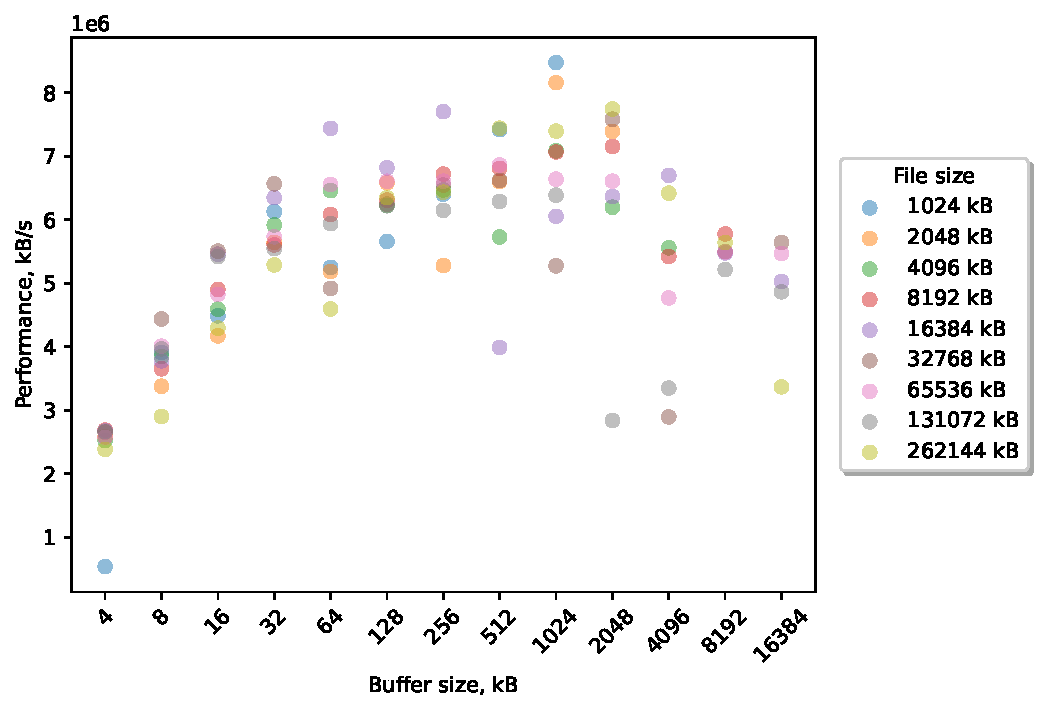
\includegraphics[width=1.0\textwidth]{figures.nosync/benchmarking/old/local/Read.pdf}
% 	\end{center}
% 	\caption{IOZone output for \gls{APFS} Forward Read}
% \end{figure}

% \begin{figure}[!htb]
% 	\label{fig:app_benapfsffs_write}
% 	\begin{center}
% 		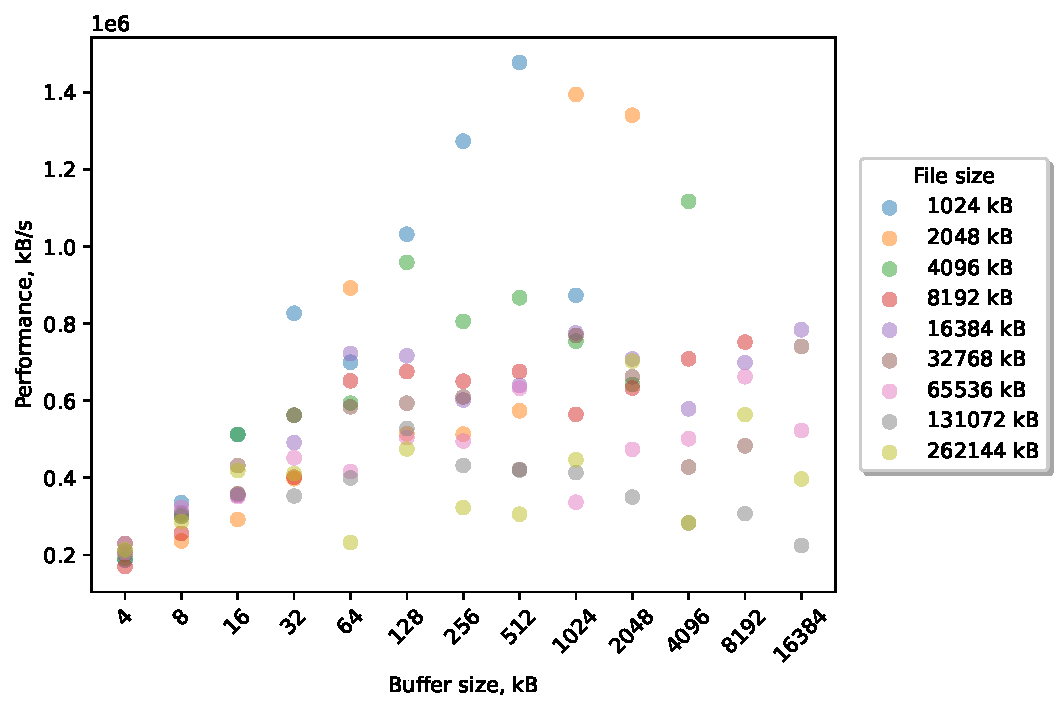
\includegraphics[width=1.0\textwidth]{figures.nosync/benchmarking/old/local/Write.pdf}
% 	\end{center}
% 	\caption{IOZone output for \gls{APFS} Forward Write}
% \end{figure}

% \begin{figure}[!htb]
% 	\label{fig:app_benchapfss_re_read}
% 	\begin{center}
% 		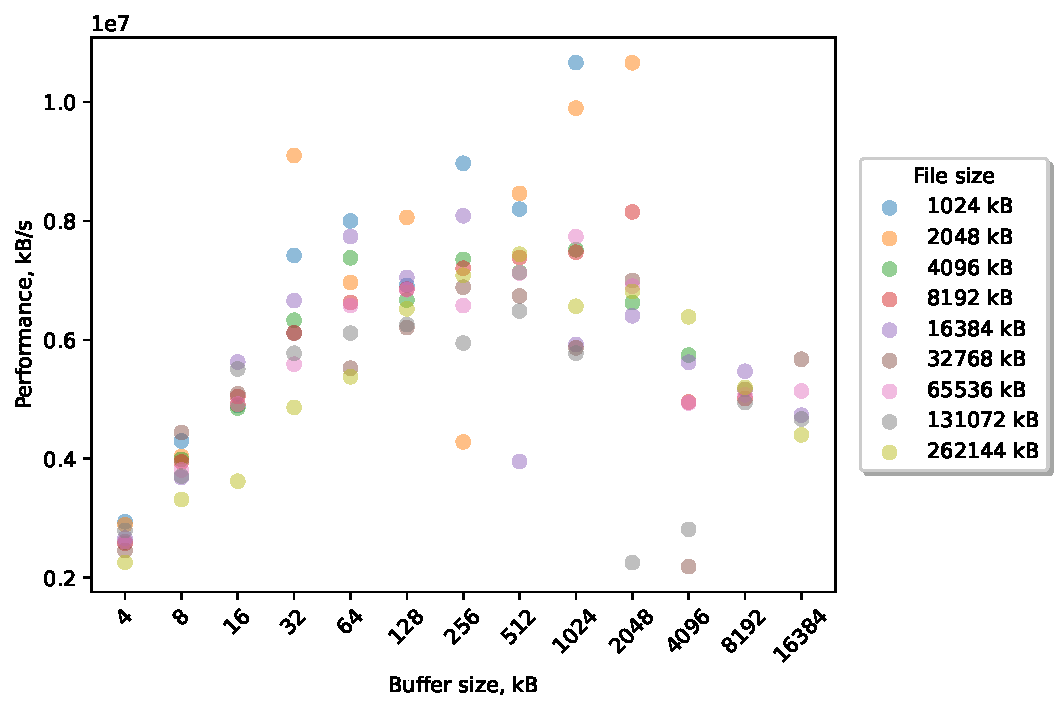
\includegraphics[width=1.0\textwidth]{figures.nosync/benchmarking/old/local/Re-Read.pdf}
% 	\end{center}
% 	\caption{IOZone output for \gls{APFS} \mbox{Re-Read}}
% \end{figure}

% \begin{figure}[!htb]
% 	\label{fig:app_bench_apfs_re_write}
% 	\begin{center}
% 		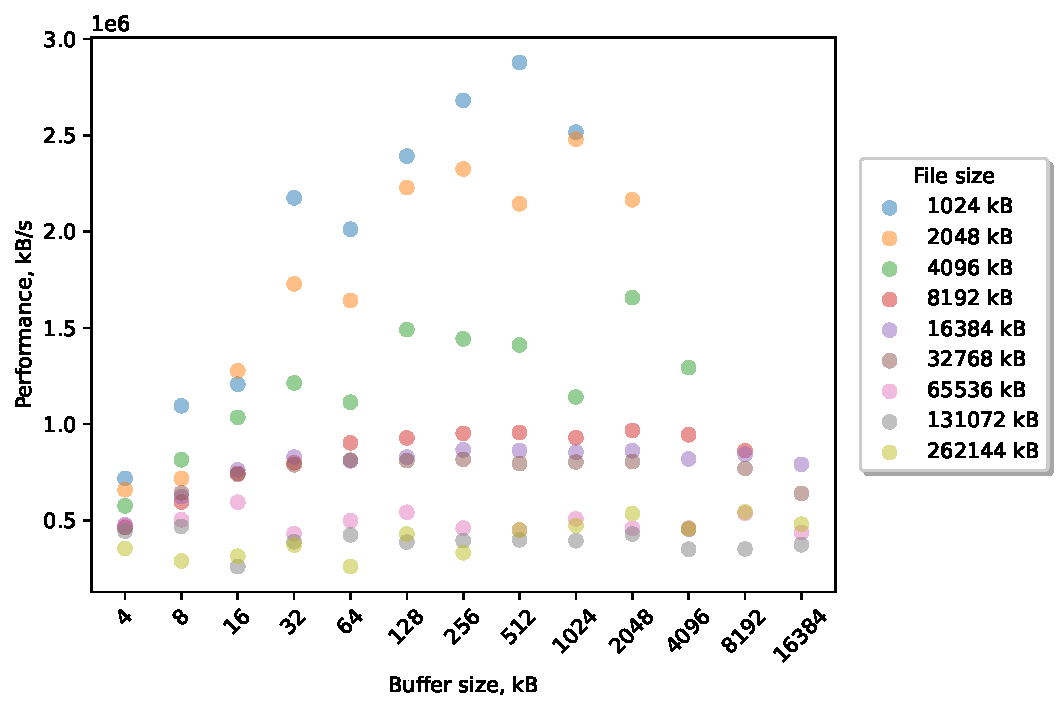
\includegraphics[width=1.0\textwidth]{figures.nosync/benchmarking/old/local/Re-Write.pdf}
% 	\end{center}
% 	\caption{IOZone output for \gls{APFS} \mbox{Re-Write}}
% \end{figure}

% \begin{figure}[!htb]
% 	\label{fig:app_bench_apfs_rnd_read}
% 	\begin{center}
% 		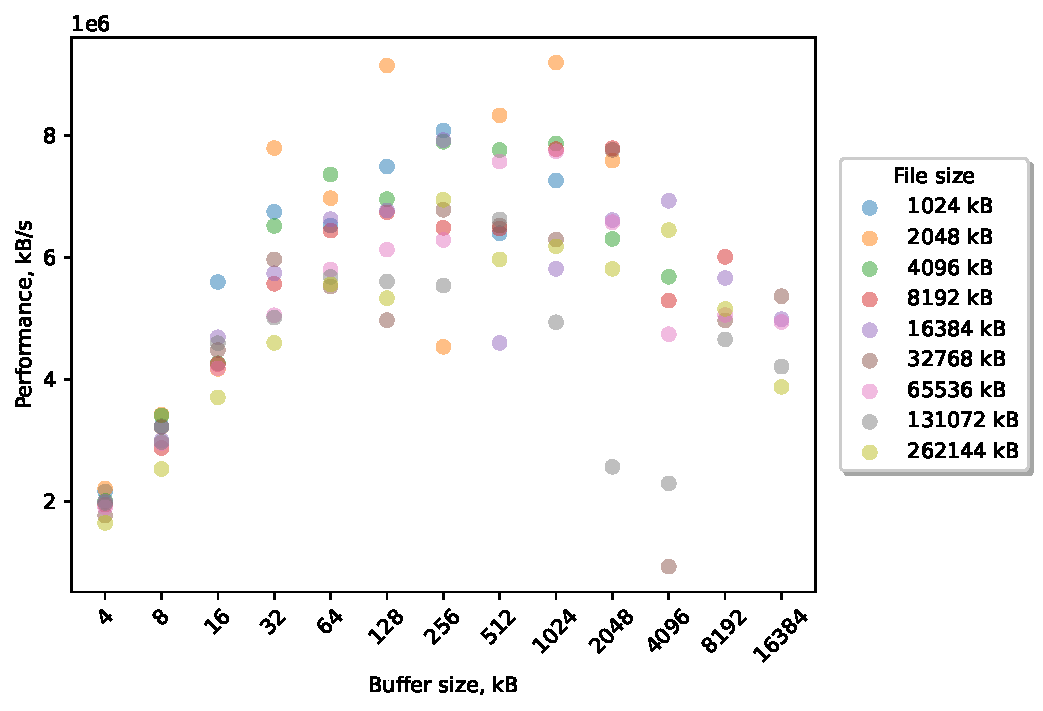
\includegraphics[width=1.0\textwidth]{figures.nosync/benchmarking/old/local/Random read.pdf}
% 	\end{center}
% 	\caption{IOZone output for \gls{APFS} Random read}
% \end{figure}

% \begin{figure}[!htb]
% 	\label{fig:app_bench_fapfsrnd_write}
% 	\begin{center}
% 		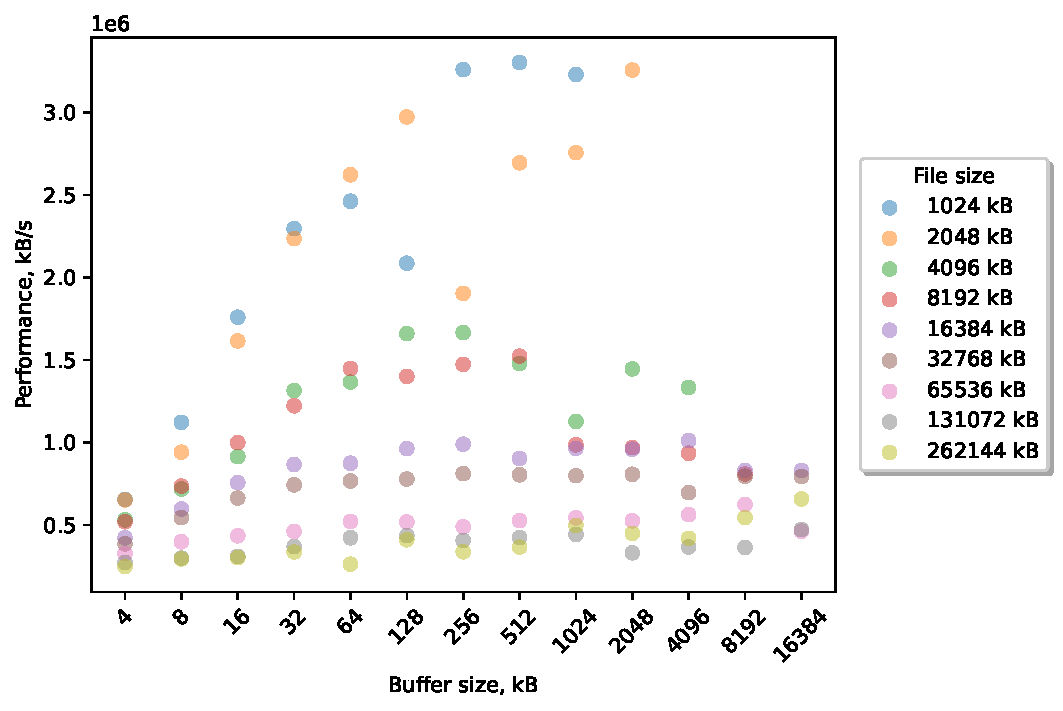
\includegraphics[width=1.0\textwidth]{figures.nosync/benchmarking/old/local/Random write.pdf}
% 	\end{center}
% 	\caption{IOZone output for \gls{APFS} Random write}
% \end{figure}